% Isosyll paper: DOPE v3 house style. Main file: paper.tex -> paper.pdf (committed).
% Build: `just paper-refresh` from the repository root (regenerates data/metrics.tex, builds PDF,
% exports docs/paper/money.png, updates README.md, and runs paper integrity tests).
% Every result number comes from data/metrics.tex (generated by python/ultra/tools/paper_data).
% Sections must not contain literal result numbers; missing metrics print a red "??" via \PH.
\documentclass[10pt,letterpaper,twocolumn]{article}
\pdfminorversion=7
% Isosyll typesetting follows the DOPE v3 technical report (e80997ba).
\usepackage[T1]{fontenc}
\usepackage[utf8]{inputenc}
\usepackage{amsmath}
\usepackage{txfonts}
\usepackage{charter}
\usepackage[scaled=0.885]{helvet}
\renewcommand{\ttdefault}{lmtt}
\usepackage[italic,defaultmathsizes]{mathastext}
\makeatletter
\DeclareSymbolFontAlphabet{\mathrm}{mtoperatorfont}
\renewcommand{\operator@font}{\mathgroup\symmtoperatorfont}
\makeatother
\usepackage[protrusion=true,expansion=true,final]{microtype}
\DisableLigatures[-]{encoding=T1,family=tt*}

\usepackage[letterpaper,left=0.80in,right=0.80in,top=0.98in,bottom=0.95in,
            columnsep=0.29in,headheight=12pt,headsep=0.30in,footskip=0.42in]{geometry}
\usepackage{graphicx}
\usepackage[table]{xcolor}
\usepackage{array,booktabs,tabularx,makecell,multirow}
\usepackage{enumitem,fancyhdr,titlesec,caption,float,stfloats,xurl}
\usepackage{tikz,pgfplots,xspace}
\pgfplotsset{compat=1.18}
\usetikzlibrary{arrows.meta,positioning,calc,fit,backgrounds,patterns,shapes.geometric}
\usepackage[numbers,sort&compress,square]{natbib}
% DOPE v3 house palette (whitepaper-v3/dope-v3.tex, e80997ba).
\definecolor{ink}{HTML}{111827}        % headings, display type
\definecolor{sub}{HTML}{4B5563}        % secondary text, captions
\definecolor{muted}{HTML}{9CA3AF}      % tertiary text
\definecolor{hair}{HTML}{D1D5DB}       % rules
\definecolor{gridline}{HTML}{E5E7EB}       % chart gridlines
\definecolor{surface}{HTML}{F3F4F6}    % neutral card
\definecolor{accent}{HTML}{D9480F}     % house orange
\definecolor{accentdark}{HTML}{B53A0B} % orange on tint
\definecolor{accenttint}{HTML}{FDEBE1}
\definecolor{blue}{HTML}{256ABF}
\definecolor{bluetint}{HTML}{EEF3FA}
\definecolor{teal}{HTML}{006D77}
\definecolor{tealtint}{HTML}{EAF4F4}
\definecolor{navy}{HTML}{1E3A5F}
\definecolor{slate}{HTML}{64748B}

% ---- links ---------------------------------------------------------------------
\usepackage[colorlinks=true,linkcolor=accent,citecolor=blue,urlcolor=blue,
            pdfusetitle,bookmarksnumbered=true]{hyperref}
\urlstyle{same}

% ---- text rhythm ---------------------------------------------------------------
\linespread{1.03}
\setlength{\parindent}{1.05em}
\setlength{\parskip}{0pt}
\emergencystretch=1.2em
\raggedbottom
% With a ragged bottom, negative penalties would end columns early before headings and lists.
\makeatletter\@secpenalty=0 \@beginparpenalty=0 \@endparpenalty=0 \@itempenalty=0 \makeatother
\clubpenalty=6000 \widowpenalty=6000
\setlist{leftmargin=1.5em,itemsep=2pt,topsep=4pt,parsep=0pt}
\renewcommand{\topfraction}{0.92}
\renewcommand{\dbltopfraction}{0.92}
\renewcommand{\bottomfraction}{0.6}
\renewcommand{\textfraction}{0.06}
\renewcommand{\floatpagefraction}{0.85}
\renewcommand{\dblfloatpagefraction}{0.85}
\setcounter{topnumber}{3}\setcounter{dbltopnumber}{3}\setcounter{totalnumber}{5}
\setlength{\textfloatsep}{14pt plus 3pt minus 2pt}
\setlength{\dbltextfloatsep}{14pt plus 3pt minus 2pt}
\setlength{\floatsep}{12pt plus 2pt minus 2pt}
\setlength{\intextsep}{10pt plus 2pt minus 2pt}

% ---- headings ------------------------------------------------------------------
\titleformat{\section}{\sffamily\bfseries\fontsize{11.6}{14}\selectfont\color{ink}\raggedright}
  {\textcolor{accent}{\thesection}}{0.62em}{}
\titlespacing*{\section}{0pt}{15pt plus 3pt minus 2pt}{5pt plus 1pt}
\titleformat{\subsection}{\sffamily\bfseries\fontsize{9.1}{11.4}\selectfont\color{ink}\raggedright}
  {\thesubsection}{0.62em}{}
\titlespacing*{\subsection}{0pt}{10pt plus 2pt minus 1pt}{3.5pt plus 1pt}
\titleformat{\subsubsection}[runin]{\normalfont\bfseries}{}{0pt}{}[.]
\titlespacing*{\subsubsection}{0pt}{6pt plus 1pt minus 1pt}{0.5em}
\newcommand{\runin}[1]{\par\smallskip\noindent\textbf{#1.}\hspace{0.45em}\ignorespaces}

\pagestyle{fancy}\fancyhf{}
\renewcommand{\headrulewidth}{0pt}\renewcommand{\footrulewidth}{0pt}
\fancyhead[L]{\sffamily\fontsize{7.4}{9}\selectfont\textcolor{sub}{\PaperTitle}}
\fancyhead[R]{\sffamily\fontsize{7.4}{9}\selectfont\textcolor{sub}{\thepage}}
\fancypagestyle{front}{\fancyhf{}%
  \fancyfoot[C]{\sffamily\fontsize{7.4}{9}\selectfont\textcolor{sub}{\thepage}}}

% ---- captions -------------------------------------------------------------------
\DeclareCaptionLabelFormat{house}{\textcolor{accent}{\bfseries #1~#2}}
\DeclareCaptionLabelSeparator{housebar}{\hspace{0.5em}\textcolor{hair}{\rule[-0.22em]{0.6pt}{1.05em}}\hspace{0.5em}}
\DeclareCaptionFont{housefont}{\sffamily\fontsize{7.9}{10.3}\selectfont\color{sub}}
\captionsetup{font=housefont,labelformat=house,labelsep=housebar,
              justification=raggedright,singlelinecheck=false,skip=6pt}
\captionsetup[table]{position=top,skip=5pt}
\newcommand{\ct}[1]{{\bfseries\color{ink}#1}}   % caption lead-in

\usepackage[capitalise,nameinlink]{cleveref}

\renewcommand{\arraystretch}{1.06}

% ---------------------------------------------------------------- placeholders and metrics
\definecolor{phred}{RGB}{200,0,0}
\newcommand{\PH}[1]{\textcolor{phred}{\textbf{??}}\ifmmode\else\fi}
\IfFileExists{data/metrics.tex}{% Generated by python/ultra/tools/paper_data. Do not edit by hand.
% Every macro is a bare number or generated sentence. Provenance: docs/paper/data/SOURCES.md.
\providecommand{\PaperMissing}[1]{\textcolor{red}{??}}
\newcommand{\PaperTitle}{Isosyll: Always Listening, Barely Computing}
\newcommand{\PaperDescriptor}{Bit-Exact Streaming Speech Recognition on One CPU Core}

\newcommand{\AbsAccuracy}{On the 730-utterance LibriSpeech DEV panel, \ultra{} v3.1.0 (final, seg.) scores 5.00\% pooled WER (3.03\% dev-clean, 7.80\% dev-other), ranking 8th of 17 complete-panel systems (lower point-estimate WER than 8 of 15 public comparators (including streaming Zipformer INT8 at 5.25\%)); \ultra{} v3.1.0 (live +LM) on the exact same INT8 weights scores 5.54\% pooled. On full LibriSpeech DEV (5,567 utt), final text reaches 5.22\% pooled (2.78\% clean / 7.82\% other; live 6.10\%). Larger models score lower at higher CPU cost on their respective timing hosts (3.56\% for Nemotron 560\,ms and 3.36\% for Parakeet TDT v3 (onnx-asr, offline)).}% [exploratory] sentence
\newcommand{\AbsParity}{Per-row centred INT8 with exact int32 accumulation and portable log-mel matches FP32 PyTorch on full DEV (5,567 utterances) within $-$0.003\,pp (95\% bounds $-$0.033 to +0.028\,pp), with repeatable, batch-invariant execution.}% [exploratory] sentence
\newcommand{\AbsSpeed}{One live stream (\ultra{} v3.1.0 (live +LM)) uses 3.1\% of one quiet Zen~2 core (32.7$\times$ real time (2.3$\times$ streaming Zipformer INT8, the fastest comparator)) and 109\,MB peak RAM ; \ultra{} v3.1.0 (final, seg.) runs at 16.8$\times$ real time and 387\,MB RAM, at 1.19x streaming Zipformer INT8's single-core speed (16.8$\times$ utterance-segmented vs. 14.0$\times$ streaming).}% [exploratory] sentence
\newcommand{\AbsWatts}{Unpaced active core energy on quiet H1 is 0.328\,J per audio-second for \ultra{} v3.1.0 (live +LM) and 0.661\,J for \ultra{} v3.1.0 (final, seg.), against 0.573\,J per audio-second for Zipformer INT8, 1.077\,J per audio-second for Moonshine Tiny, 1.711\,J per audio-second for Parakeet TDT v3 (sherpa-onnx, offline) and 4.513\,J per audio-second for Nemotron 560\,ms (quiet 73-clip timing) (CPU domain only, not wall power).}% [exploratory] sentence
\newcommand{\AudioHSixtyOneCleanDelta}{+0.223}% [exploratory] percentage points
\newcommand{\AudioHSixtyOneCleanFixed}{+0.331}% [exploratory] percentage points
\newcommand{\AudioHSixtyOneCleanJoint}{+0.344}% [exploratory] percentage points
\newcommand{\AudioHSixtyOneNoiseDelta}{$-$0.114}% [exploratory] percentage points
\newcommand{\AudioHSixtyOneNoiseFixed}{$-$0.010}% [exploratory] percentage points
\newcommand{\AudioHSixtyOneNoiseJoint}{+0.016}% [exploratory] percentage points
\newcommand{\AudioHSixtyOneNoisePython}{$-$8.853}% [exploratory] percentage points
\newcommand{\AudioMOneFourDelta}{$-$0.052}% [exploratory] percentage points
\newcommand{\AudioMOneFourUpper}{+0.044}% [exploratory] percentage points
\newcommand{\AudioProbeAgcBar}{0.087}% [exploratory] percentage points
\newcommand{\AudioProbeAgcCalDelta}{+0.032}% [exploratory] percentage points
\newcommand{\AudioProbeAgcCalRepeat}{11}% [exploratory] inserted repeats
\newcommand{\AudioProbeAgcDelta}{+0.091}% [exploratory] percentage points
\newcommand{\AudioProbeAgcRepeatOff}{8}% [exploratory] inserted repeats
\newcommand{\AudioProbeAgcRepeatOn}{9}% [exploratory] inserted repeats
\newcommand{\AudioProbeMusanGain}{$-$0.455}% [exploratory] percentage points
\newcommand{\AudioProbeTokenBar}{0.30}% [exploratory] Youden J
\newcommand{\AudioProbeTokenYouden}{0.095}% [exploratory] Youden J
\newcommand{\AudioProbeWhiteGain}{$-$0.934}% [exploratory] percentage points
\newcommand{\AudioZOneAutoCleanDelta}{$-$0.08}% [exploratory] percentage points
\newcommand{\AudioZOneAutoCleanUpper}{$-$0.02}% [exploratory] percentage points
\newcommand{\AudioZOneAutoThirtyDelta}{$-$3.36}% [exploratory] percentage points
\newcommand{\AudioZOneAutoThirtyUpper}{$-$2.98}% [exploratory] percentage points
\newcommand{\AudioZOneAutoTwentyDelta}{$-$1.73}% [exploratory] percentage points
\newcommand{\AudioZOneAutoTwentyUpper}{$-$1.51}% [exploratory] percentage points
\newcommand{\AudioZOneCleanDelta}{$-$0.022}% [exploratory] percentage points
\newcommand{\AudioZOneCleanUpper}{+0.028}% [exploratory] percentage points
\newcommand{\AudioZOneCpuEngineUpper}{+0.21}% [exploratory] % relative CPU
\newcommand{\AudioZOneCpuStreamUpper}{+0.31}% [exploratory] % relative CPU
\newcommand{\AudioZOneCrossIsaClips}{50}% [exploratory] clips
\newcommand{\AudioZOneCrossIsaCommit}{f04027c}% [exploratory] commit
\newcommand{\AudioZOneCrossIsaDiffs}{0}% [exploratory] differing clips
\newcommand{\AudioZOneOracleTupleDiffs}{5}% [exploratory] clips with full-tuple diffs
\newcommand{\AudioZOneThirtyDelta}{$-$0.943}% [exploratory] percentage points
\newcommand{\AudioZOneThirtyUpper}{$-$0.723}% [exploratory] percentage points
\newcommand{\AudioZOneTwentyDelta}{$-$0.175}% [exploratory] percentage points
\newcommand{\AudioZOneTwentyUpper}{$-$0.044}% [exploratory] percentage points
\newcommand{\CandCUtts}{2785}% [exploratory] utterances
\newcommand{\CandFinalCDelta}{$-$0.11}% [exploratory] pp WER
\newcommand{\CandFinalCHi}{+0.11}% [exploratory] pp WER
\newcommand{\CandFinalCLo}{$-$0.35}% [exploratory] pp WER
\newcommand{\CandFinalEdits}{722}% [exploratory] edits
\newcommand{\CandFinalFullClean}{2.78}% [exploratory] % WER
\newcommand{\CandFinalFullEdits}{5540}% [exploratory] edits
\newcommand{\CandFinalFullOther}{7.82}% [exploratory] % WER
\newcommand{\CandFinalFullWer}{5.22}% [exploratory] % WER
\newcommand{\CandFinalLowmemCDelta}{$-$0.10}% [exploratory] pp WER
\newcommand{\CandFinalLowmemCHi}{+0.12}% [exploratory] pp WER
\newcommand{\CandFinalLowmemCLo}{$-$0.35}% [exploratory] pp WER
\newcommand{\CandFinalLowmemEdits}{735}% [exploratory] edits
\newcommand{\CandFinalLowmemFullClean}{2.84}% [exploratory] % WER
\newcommand{\CandFinalLowmemFullOther}{7.79}% [exploratory] % WER
\newcommand{\CandFinalLowmemFullWer}{5.24}% [exploratory] % WER
\newcommand{\CandFinalLowmemPanelDelta}{$-$0.17}% [exploratory] pp WER
\newcommand{\CandFinalLowmemPanelHi}{+0.15}% [exploratory] pp WER
\newcommand{\CandFinalLowmemPanelLo}{$-$0.49}% [exploratory] pp WER
\newcommand{\CandFinalLowmemWer}{5.09}% [exploratory] % WER
\newcommand{\CandFinalOldDelta}{$-$0.06}% [exploratory] pp WER
\newcommand{\CandFinalOldHi}{+0.17}% [exploratory] pp WER
\newcommand{\CandFinalOldLo}{$-$0.28}% [exploratory] pp WER
\newcommand{\CandFinalPanelDelta}{$-$0.26}% [exploratory] pp WER
\newcommand{\CandFinalPanelHi}{+0.05}% [exploratory] pp WER
\newcommand{\CandFinalPanelLo}{$-$0.57}% [exploratory] pp WER
\newcommand{\CandFinalWer}{5.00}% [exploratory] % WER
\newcommand{\CandFullCleanUtts}{2703}% [exploratory] utterances
\newcommand{\CandFullOtherUtts}{2864}% [exploratory] utterances
\newcommand{\CandGateFinalFull}{5489}% [exploratory] edits
\newcommand{\CandGateFinalPanel}{650}% [exploratory] edits
\newcommand{\CandGateLivePanel}{722}% [exploratory] edits
\newcommand{\CandHolmFinal}{0.27}% [exploratory] p
\newcommand{\CandHolmNi}{0.27}% [exploratory] p
\newcommand{\CandHolmOld}{0.33}% [exploratory] p
\newcommand{\CandIsaRuns}{18}% [exploratory] runs
\newcommand{\CandLiveGreedyCDelta}{+1.59}% [exploratory] pp WER
\newcommand{\CandLiveGreedyCHi}{+1.90}% [exploratory] pp WER
\newcommand{\CandLiveGreedyCLo}{+1.31}% [exploratory] pp WER
\newcommand{\CandLiveGreedyEdits}{900}% [exploratory] edits
\newcommand{\CandLiveGreedyFullClean}{3.66}% [exploratory] % WER
\newcommand{\CandLiveGreedyFullOther}{10.22}% [exploratory] % WER
\newcommand{\CandLiveGreedyFullWer}{6.83}% [exploratory] % WER
\newcommand{\CandLiveGreedyOldDelta}{$-$0.62}% [exploratory] pp WER
\newcommand{\CandLiveGreedyOldHi}{$-$0.38}% [exploratory] pp WER
\newcommand{\CandLiveGreedyOldLo}{$-$0.86}% [exploratory] pp WER
\newcommand{\CandLiveGreedyPanelDelta}{+0.98}% [exploratory] pp WER
\newcommand{\CandLiveGreedyPanelHi}{+1.29}% [exploratory] pp WER
\newcommand{\CandLiveGreedyPanelLo}{+0.66}% [exploratory] pp WER
\newcommand{\CandLiveGreedyWer}{6.23}% [exploratory] % WER
\newcommand{\CandLiveLmCDelta}{+0.81}% [exploratory] pp WER
\newcommand{\CandLiveLmCHi}{+1.02}% [exploratory] pp WER
\newcommand{\CandLiveLmCLo}{+0.62}% [exploratory] pp WER
\newcommand{\CandLiveLmEdits}{800}% [exploratory] edits
\newcommand{\CandLiveLmEightCDelta}{+0.65}% [exploratory] pp WER
\newcommand{\CandLiveLmEightCHi}{+0.84}% [exploratory] pp WER
\newcommand{\CandLiveLmEightCLo}{+0.47}% [exploratory] pp WER
\newcommand{\CandLiveLmEightEdits}{794}% [exploratory] edits
\newcommand{\CandLiveLmEightFullClean}{3.12}% [exploratory] % WER
\newcommand{\CandLiveLmEightFullOther}{8.79}% [exploratory] % WER
\newcommand{\CandLiveLmEightFullWer}{5.87}% [exploratory] % WER
\newcommand{\CandLiveLmEightOldDelta}{$-$1.35}% [exploratory] pp WER
\newcommand{\CandLiveLmEightOldHi}{$-$1.03}% [exploratory] pp WER
\newcommand{\CandLiveLmEightOldLo}{$-$1.68}% [exploratory] pp WER
\newcommand{\CandLiveLmEightPanelDelta}{+0.24}% [exploratory] pp WER
\newcommand{\CandLiveLmEightPanelHi}{+0.52}% [exploratory] pp WER
\newcommand{\CandLiveLmEightPanelLo}{$-$0.04}% [exploratory] pp WER
\newcommand{\CandLiveLmEightWer}{5.50}% [exploratory] % WER
\newcommand{\CandLiveLmFullClean}{3.25}% [exploratory] % WER
\newcommand{\CandLiveLmFullOther}{9.13}% [exploratory] % WER
\newcommand{\CandLiveLmFullWer}{6.10}% [exploratory] % WER
\newcommand{\CandLiveLmOldDelta}{$-$1.31}% [exploratory] pp WER
\newcommand{\CandLiveLmOldHi}{$-$1.00}% [exploratory] pp WER
\newcommand{\CandLiveLmOldLo}{$-$1.63}% [exploratory] pp WER
\newcommand{\CandLiveLmPanelDelta}{+0.28}% [exploratory] pp WER
\newcommand{\CandLiveLmPanelHi}{+0.58}% [exploratory] pp WER
\newcommand{\CandLiveLmPanelLo}{$-$0.02}% [exploratory] pp WER
\newcommand{\CandLiveLmWer}{5.54}% [exploratory] % WER
\newcommand{\CandNiMargin}{0.50}% [exploratory] pp
\newcommand{\CandTrainKh}{276{,}863}% [exploratory] audio-h
\newcommand{\CandZipCWer}{5.13}% [exploratory] % WER
\newcommand{\CandZipFullWer}{5.37}% [exploratory] % WER
\newcommand{\ColdAbstractFinal}{The full live-plus-commit pipeline, committing at reference utterance boundaries, reaches 5.00\% pooled WER at 16.8$\times$ real time.}% [exploratory] sentence
\newcommand{\ColdAbstractLive}{Live decoding runs at 32.7$\times$ real time with 109\,MB peak RSS, 0.328\,J active core energy per audio-second, and 5.54\% pooled WER.}% [exploratory] sentence
\newcommand{\ColdAbstractMoreAcc}{Seven of the 15 public recognisers we measured are more accurate than the final mode.}% [reported] sentence
\newcommand{\ColdAbstractZip}{Streaming Zipformer INT8 reaches 14.0$\times$ real time and 5.25\% WER under the matched protocol; Isosyll live delivers 2.3$\times$ its throughput at 57\% of its active core energy.}% [exploratory] sentence
\newcommand{\ColdAccuracyCount}{7}% [reported] rows
\newcommand{\ColdAccuracySentence}{\ultra{} v3.1.0 (final, seg.) (5.00\% pooled) ranks 8th of 17 complete-panel systems (lower point-estimate WER than 8 of 15 public comparators, including streaming Zipformer INT8 at 5.25\%). 7 of the 15 comparators achieve lower pooled WER. Among configurations with plotted throughput, Parakeet TDT v3 (onnx-asr, offline) has the lowest pooled WER at 3.36\% (2.52\% dev-clean, 4.58\% dev-other), 1.63 points below \ultra{} v3.1.0 (final, seg.).}% [reported] sentence
\newcommand{\ColdAnchorCount}{0}% [reported] rows
\newcommand{\ColdAnchorSentence}{No system has a quiet second measurement yet, so there is no host-agreement check.}% [reported] sentence
\newcommand{\ColdAudioMinutes}{87.7}% [reported] minutes of audio
\newcommand{\ColdComparatorCount}{12}% [reported] rows
\newcommand{\ColdCompleteCompCount}{15}% [reported] rows
\newcommand{\ColdCompletePanelCount}{17}% [reported] rows
\newcommand{\ColdConclusionResult}{two operating points on one INT8 artifact: 32.7$\times$ real-time continuous live streaming at 0.328\,J per audio-second and 109\,MB RAM (5.54\% panel WER), and an utterance-segmented commit pass reaching 5.00\% pooled panel WER (5.22\% on full DEV) at 16.8$\times$ real time (387\,MB RAM, 0.661\,J per audio-second, commit delay not re-measured)---at 1.19$\times$ streaming Zipformer INT8's single-core speed (16.8$\times$ utterance-segmented vs.\ 14.0$\times$ streaming) at 5.00\% vs.\ 5.25\% pooled WER}% [reported] sentence
\newcommand{\ColdFinalCorePct}{5.9}% [exploratory] % of one core
\newcommand{\ColdFinalVsZipSpeed}{at 1.19$\times$ streaming Zipformer INT8's single-core speed (16.8$\times$ utterance-segmented vs.\ 14.0$\times$ streaming)}% [reported] sentence
\newcommand{\ColdHeadCorePct}{3.1}% [exploratory] % of one core
\newcommand{\ColdHeadCpu}{0.059}% [exploratory] CPU-s/audio-s
\newcommand{\ColdHeadModel}{60}% [exploratory] MB of model files
\newcommand{\ColdHeadRss}{387}% [exploratory] MB peak resident memory
\newcommand{\ColdHeadSentence}{On one quiet Zen~2 core (host H1), \ultra{} v3.1.0 (live +LM) decodes cold at 32.7$\times$ real time (3.1\% of one core, 109\,MB peak memory) at 5.54\% pooled panel WER (3.20\% dev-clean, 8.88\% dev-other). Adding the utterance-segmented commit pass on the same weights (\ultra{} v3.1.0 (final, seg.)) runs cold at 16.8$\times$ real time (387\,MB peak memory) and reaches pooled panel WER 5.00\% (3.03\% dev-clean, 7.80\% dev-other).}% [reported] sentence
\newcommand{\ColdHeadSpeed}{16.8}% [exploratory] x real time, one core
\newcommand{\ColdHeadSpeedOverFast}{2.3}% [exploratory] x
\newcommand{\ColdHeadWatts}{0.661}% [exploratory] W per stream (live + commit)
\newcommand{\ColdHeadWer}{5.00}% [exploratory] % WER, pooled
\newcommand{\ColdHeadWerBeaten}{8}% [reported] rows
\newcommand{\ColdHeadWerClean}{3.03}% [exploratory] % WER, dev-clean half
\newcommand{\ColdHeadWerGapBest}{1.63}% [exploratory] pp WER
\newcommand{\ColdHeadWerOther}{7.80}% [exploratory] % WER, dev-other half
\newcommand{\ColdHeadWerRank}{8}% [reported] rows
\newcommand{\ColdHeadWerRankOrd}{8th}% [reported] sentence
\newcommand{\ColdHostAbstract}{3 of the 14 systems are still measured on a shared host; quiet-host rows replace them as they arrive.}% [reported] sentence
\newcommand{\ColdHostSentence}{3 of the 14 points are still interim (lighter marks): measured on host H0, a shared host that ran other jobs and makes every system slower, until their rows from the quiet host H1 arrive.}% [reported] sentence
\newcommand{\ColdHostShort}{Lighter marks (3 of 14 points): interim, measured on the shared host H0 until their quiet-host (H1) rows arrive.}% [reported] sentence
\newcommand{\ColdIntroContrib}{Live streaming on one quiet Zen~2 core (32.7$\times$ vs.\ 14.0$\times$ for Zipformer INT8, 2.3$\times$; 0.328\,J per audio-second; 109\,MB RAM; 5.54\% pooled panel WER), paired on the same INT8 weights with an utterance-segmented commit pass (16.8$\times$, 0.661\,J per audio-second, 387\,MB RAM) that reaches 5.00\% pooled panel WER against 5.25\% for streaming Zipformer INT8 (paired comparison in \cref{sec:versus}), at 1.19$\times$ streaming Zipformer INT8's single-core speed.}% [reported] sentence
\newcommand{\ColdIntroLiveItem}{160\,ms chunked decoding with a 34.5\,MiB live language model with no endpoint detector required, using 3.1\% of one quiet Zen~2 core (32.7$\times$ real time, 109\,MB peak RAM, 0.328\,J per audio-second of active core energy)---2.3$\times$ the throughput of matched streaming Zipformer INT8 at 57\% of its active core energy per audio-second---at 5.54\% pooled panel WER (6.10\% full DEV).}% [reported] sentence
\newcommand{\ColdLightRssOverHead}{1.4}% [exploratory] x
\newcommand{\ColdLimitLive}{While \ultra{} v3.1.0 (live +LM) streams continuously at 32.7$\times$ real time, 0.328\,J per audio-second, and 109\,MB RAM without an endpoint detector, the higher-accuracy \ultra{} v3.1.0 (final, seg.) operating point requires utterance endpoints (capped at 40\,s), adds a post-endpoint commit delay (median 211\,ms measured on the prior release, not re-measured), and increases peak RSS to 387\,MB due to the 5-gram LM pack.}% [reported] sentence
\newcommand{\ColdLiveCpu}{0.031}% [exploratory] CPU-s/audio-s
\newcommand{\ColdLiveModel}{60}% [exploratory] MB of model files
\newcommand{\ColdLiveRss}{109}% [exploratory] MB peak resident memory
\newcommand{\ColdLiveSpeed}{32.7}% [exploratory] x real time, one core
\newcommand{\ColdLiveWatts}{0.328}% [exploratory] W per live stream
\newcommand{\ColdLiveWer}{5.54}% [exploratory] % WER, pooled
\newcommand{\ColdLiveWerClean}{3.20}% [exploratory] % WER, dev-clean half
\newcommand{\ColdLiveWerOther}{8.88}% [exploratory] % WER, dev-other half
\newcommand{\ColdMemorySentence}{In live mode, \ultra{} peaks at 109\,MB, 72\% of matched streaming Zipformer INT8 (152\,MB) and 69.7$\times$ less than Vosk Large (7629\,MB, timed separately); loading the larger 5-gram LM for the commit pass raises peak RSS to 387\,MB.}% [reported] sentence
\newcommand{\ColdMoonSmallCorePct}{49.5}% [exploratory] % of one core for one always-on stream
\newcommand{\ColdMoonSmallCpu}{0.495}% [exploratory] CPU-s/audio-s
\newcommand{\ColdMoonSmallModel}{142}% [exploratory] MB of model files (10^6 bytes)
\newcommand{\ColdMoonSmallRss}{476}% [exploratory] MB peak resident memory of the process tree (10^6 bytes)
\newcommand{\ColdMoonSmallRtfx}{2.02}% [exploratory] audio-s per wall-s
\newcommand{\ColdMoonSmallSpeed}{2.02}% [exploratory] audio-s per CPU-s (x real time on the pinned cores)
\newcommand{\ColdMoonSmallWer}{5.93}% [exploratory] % WER
\newcommand{\ColdMoonSmallWerClean}{3.98}% [exploratory] % WER
\newcommand{\ColdMoonSmallWerOther}{8.73}% [exploratory] % WER
\newcommand{\ColdMoonTinyCorePct}{12.2}% [exploratory] % of one core for one always-on stream
\newcommand{\ColdMoonTinyCpu}{0.122}% [exploratory] CPU-s/audio-s
\newcommand{\ColdMoonTinyModel}{45}% [exploratory] MB of model files (10^6 bytes)
\newcommand{\ColdMoonTinyRss}{201}% [exploratory] MB peak resident memory of the process tree (10^6 bytes)
\newcommand{\ColdMoonTinyRtfx}{8.19}% [exploratory] audio-s per wall-s
\newcommand{\ColdMoonTinySpeed}{8.20}% [exploratory] audio-s per CPU-s (x real time on the pinned cores)
\newcommand{\ColdMoonTinyWatts}{1.077}% [exploratory] W per live stream (= J per audio-s)
\newcommand{\ColdMoonTinyWer}{9.90}% [exploratory] % WER
\newcommand{\ColdMoonTinyWerClean}{6.54}% [exploratory] % WER
\newcommand{\ColdMoonTinyWerOther}{14.72}% [exploratory] % WER
\newcommand{\ColdNemoFiveSixtyCorePct}{42.0}% [exploratory] % of one core for one always-on stream
\newcommand{\ColdNemoFiveSixtyCpu}{0.420}% [exploratory] CPU-s/audio-s
\newcommand{\ColdNemoFiveSixtyModel}{700}% [exploratory] MB of model files (10^6 bytes)
\newcommand{\ColdNemoFiveSixtyRss}{987}% [exploratory] MB peak resident memory of the process tree (10^6 bytes)
\newcommand{\ColdNemoFiveSixtyRtfx}{2.38}% [exploratory] audio-s per wall-s
\newcommand{\ColdNemoFiveSixtySpeed}{2.38}% [exploratory] audio-s per CPU-s (x real time on the pinned cores)
\newcommand{\ColdNemoFiveSixtyWatts}{4.513}% [exploratory] W per live stream (= J per audio-s)
\newcommand{\ColdNemoFiveSixtyWer}{3.56}% [exploratory] % WER
\newcommand{\ColdNemoFiveSixtyWerClean}{2.61}% [exploratory] % WER
\newcommand{\ColdNemoFiveSixtyWerOther}{4.93}% [exploratory] % WER
\newcommand{\ColdNemoOneSixtyCorePct}{78.2}% [exploratory] % of one core for one always-on stream
\newcommand{\ColdNemoOneSixtyCpu}{0.782}% [exploratory] CPU-s/audio-s
\newcommand{\ColdNemoOneSixtyModel}{700}% [exploratory] MB of model files (10^6 bytes)
\newcommand{\ColdNemoOneSixtyRss}{1287}% [exploratory] MB peak resident memory of the process tree (10^6 bytes)
\newcommand{\ColdNemoOneSixtyRtfx}{1.28}% [exploratory] audio-s per wall-s
\newcommand{\ColdNemoOneSixtySpeed}{1.28}% [exploratory] audio-s per CPU-s (x real time on the pinned cores)
\newcommand{\ColdNemoOneSixtyWer}{3.94}% [exploratory] % WER
\newcommand{\ColdNemoOneSixtyWerClean}{2.90}% [exploratory] % WER
\newcommand{\ColdNemoOneSixtyWerOther}{5.42}% [exploratory] % WER
\newcommand{\ColdNemoThreeFiveCorePct}{118.6}% [exploratory] % of one core for one always-on stream
\newcommand{\ColdNemoThreeFiveCpu}{1.186}% [exploratory] CPU-s/audio-s
\newcommand{\ColdNemoThreeFiveModel}{742}% [exploratory] MB of model files (10^6 bytes)
\newcommand{\ColdNemoThreeFiveRss}{1277}% [exploratory] MB peak resident memory of the process tree (10^6 bytes)
\newcommand{\ColdNemoThreeFiveRtfx}{0.84}% [exploratory] audio-s per wall-s
\newcommand{\ColdNemoThreeFiveSpeed}{0.84}% [exploratory] audio-s per CPU-s (x real time on the pinned cores)
\newcommand{\ColdNemoThreeFiveWer}{6.14}% [exploratory] % WER
\newcommand{\ColdNemoThreeFiveWerClean}{4.14}% [exploratory] % WER
\newcommand{\ColdNemoThreeFiveWerOther}{9.00}% [exploratory] % WER
\newcommand{\ColdOrderSentence}{The dev-other split changes the rank order of 6 systems relative to dev-clean (notably the \ultra{} final mode has lower dev-other WER than Zipformer INT8).}% [reported] sentence
\newcommand{\ColdParakeetOnnxAsrCorePct}{15.0}% [exploratory] % of one core for one always-on stream
\newcommand{\ColdParakeetOnnxAsrCpu}{0.150}% [exploratory] CPU-s/audio-s
\newcommand{\ColdParakeetOnnxAsrModel}{670}% [exploratory] MB of model files (10^6 bytes)
\newcommand{\ColdParakeetOnnxAsrRss}{1684}% [exploratory] MB peak resident memory of the process tree (10^6 bytes)
\newcommand{\ColdParakeetOnnxAsrRtfx}{6.68}% [exploratory] audio-s per wall-s
\newcommand{\ColdParakeetOnnxAsrSpeed}{6.69}% [exploratory] audio-s per CPU-s (x real time on the pinned cores)
\newcommand{\ColdParakeetOnnxAsrWer}{3.36}% [exploratory] % WER
\newcommand{\ColdParakeetOnnxAsrWerClean}{2.52}% [exploratory] % WER
\newcommand{\ColdParakeetOnnxAsrWerOther}{4.58}% [exploratory] % WER
\newcommand{\ColdParakeetTdtCorePct}{16.9}% [exploratory] % of one core for one always-on stream
\newcommand{\ColdParakeetTdtCpu}{0.169}% [exploratory] CPU-s/audio-s
\newcommand{\ColdParakeetTdtModel}{671}% [exploratory] MB of model files (10^6 bytes)
\newcommand{\ColdParakeetTdtRss}{1403}% [exploratory] MB peak resident memory of the process tree (10^6 bytes)
\newcommand{\ColdParakeetTdtRtfx}{5.91}% [exploratory] audio-s per wall-s
\newcommand{\ColdParakeetTdtSpeed}{5.92}% [exploratory] audio-s per CPU-s (x real time on the pinned cores)
\newcommand{\ColdParakeetTdtWatts}{1.711}% [exploratory] W per live stream (= J per audio-s)
\newcommand{\ColdParakeetTdtWer}{3.40}% [exploratory] % WER
\newcommand{\ColdParakeetTdtWerClean}{2.43}% [exploratory] % WER
\newcommand{\ColdParakeetTdtWerOther}{4.78}% [exploratory] % WER
\newcommand{\ColdRcTwoFinalCorePct}{5.9}% [exploratory] % of one core for one always-on stream
\newcommand{\ColdRcTwoFinalCpu}{0.059}% [exploratory] CPU-s/audio-s
\newcommand{\ColdRcTwoFinalModel}{60}% [exploratory] MB of model files (10^6 bytes)
\newcommand{\ColdRcTwoFinalRss}{387}% [exploratory] MB peak resident memory of the process tree (10^6 bytes)
\newcommand{\ColdRcTwoFinalRtfx}{16.8}% [exploratory] audio-s per wall-s
\newcommand{\ColdRcTwoFinalSpeed}{16.8}% [exploratory] audio-s per CPU-s (x real time on the pinned cores)
\newcommand{\ColdRcTwoFinalWatts}{0.661}% [exploratory] W per live stream (= J per audio-s)
\newcommand{\ColdRcTwoFinalWer}{5.00}% [exploratory] % WER
\newcommand{\ColdRcTwoFinalWerClean}{3.03}% [exploratory] % WER
\newcommand{\ColdRcTwoFinalWerOther}{7.80}% [exploratory] % WER
\newcommand{\ColdRcTwoLiveGreedyCorePct}{2.9}% [exploratory] % of one core for one always-on stream
\newcommand{\ColdRcTwoLiveGreedyCpu}{0.029}% [exploratory] CPU-s/audio-s
\newcommand{\ColdRcTwoLiveGreedyModel}{60}% [exploratory] MB of model files (10^6 bytes)
\newcommand{\ColdRcTwoLiveGreedyRss}{74}% [exploratory] MB peak resident memory of the process tree (10^6 bytes)
\newcommand{\ColdRcTwoLiveGreedyRtfx}{34.2}% [exploratory] audio-s per wall-s
\newcommand{\ColdRcTwoLiveGreedySpeed}{34.2}% [exploratory] audio-s per CPU-s (x real time on the pinned cores)
\newcommand{\ColdRcTwoLiveGreedyWatts}{0.322}% [exploratory] W per live stream (= J per audio-s)
\newcommand{\ColdRcTwoLiveGreedyWer}{6.23}% [exploratory] % WER
\newcommand{\ColdRcTwoLiveGreedyWerClean}{3.68}% [exploratory] % WER
\newcommand{\ColdRcTwoLiveGreedyWerOther}{9.87}% [exploratory] % WER
\newcommand{\ColdRcTwoLiveLmCorePct}{3.1}% [exploratory] % of one core for one always-on stream
\newcommand{\ColdRcTwoLiveLmCpu}{0.031}% [exploratory] CPU-s/audio-s
\newcommand{\ColdRcTwoLiveLmModel}{60}% [exploratory] MB of model files (10^6 bytes)
\newcommand{\ColdRcTwoLiveLmRss}{109}% [exploratory] MB peak resident memory of the process tree (10^6 bytes)
\newcommand{\ColdRcTwoLiveLmRtfx}{32.7}% [exploratory] audio-s per wall-s
\newcommand{\ColdRcTwoLiveLmSpeed}{32.7}% [exploratory] audio-s per CPU-s (x real time on the pinned cores)
\newcommand{\ColdRcTwoLiveLmWatts}{0.328}% [exploratory] W per live stream (= J per audio-s)
\newcommand{\ColdRcTwoLiveLmWer}{5.54}% [exploratory] % WER
\newcommand{\ColdRcTwoLiveLmWerClean}{3.20}% [exploratory] % WER
\newcommand{\ColdRcTwoLiveLmWerOther}{8.88}% [exploratory] % WER
\newcommand{\ColdRcTwoLiveLmWideCorePct}{3.0}% [exploratory] % of one core for one always-on stream
\newcommand{\ColdRcTwoLiveLmWideCpu}{0.030}% [exploratory] CPU-s/audio-s
\newcommand{\ColdRcTwoLiveLmWideModel}{60}% [exploratory] MB of model files (10^6 bytes)
\newcommand{\ColdRcTwoLiveLmWideRss}{111}% [exploratory] MB peak resident memory of the process tree (10^6 bytes)
\newcommand{\ColdRcTwoLiveLmWideRtfx}{33.3}% [exploratory] audio-s per wall-s
\newcommand{\ColdRcTwoLiveLmWideSpeed}{33.3}% [exploratory] audio-s per CPU-s (x real time on the pinned cores)
\newcommand{\ColdRcTwoLiveLmWideWatts}{0.316}% [exploratory] W per live stream (= J per audio-s)
\newcommand{\ColdRcTwoLiveLmWideWer}{5.50}% [exploratory] % WER
\newcommand{\ColdRcTwoLiveLmWideWerClean}{3.27}% [exploratory] % WER
\newcommand{\ColdRcTwoLiveLmWideWerOther}{8.68}% [exploratory] % WER
\newcommand{\ColdRowsCount}{14}% [reported] rows
\newcommand{\ColdRowsEnergy}{6}% [reported] rows
\newcommand{\ColdRowsFaded}{3}% [reported] rows
\newcommand{\ColdRowsInterim}{3}% [reported] rows
\newcommand{\ColdRowsLag}{0}% [reported] rows
\newcommand{\ColdRowsOffFrontier}{3}% [reported] rows
\newcommand{\ColdRowsStreaming}{12}% [reported] rows
\newcommand{\ColdRowsSubset}{4}% [reported] rows
\newcommand{\ColdRowsUndrawn}{1}% [reported] rows
\newcommand{\ColdRowsWhole}{2}% [reported] rows
\newcommand{\ColdSpeedSentence}{On the quiet full-panel host H1, \ultra{} v3.1.0 (live +LM) runs at 32.7$\times$ against 14.0$\times$ for matched streaming Zipformer INT8 (2.3$\times$), while utterance-segmented \ultra{} v3.1.0 (final, seg.) runs at 1.19$\times$ streaming Zipformer INT8's single-core speed (16.8$\times$ utterance-segmented vs.\ 14.0$\times$ streaming).}% [reported] sentence
\newcommand{\ColdSubsetSentence}{4 slow systems are timed on a 73-utterance subset of the panel (Nemotron 560\,ms, Vosk Large, Whisper.cpp Tiny and Whisper.cpp Base); their WER is from the full panel.}% [reported] sentence
\newcommand{\ColdSubtitle}{Live: 32.7$\times$ real time, 5.54\% WER $\cdot$ Final (commit pass at utterance ends): 16.8$\times$, 5.00\% WER}% [exploratory] sentence
\newcommand{\ColdUltraFinalCorePct}{7.1}% [exploratory] % of one core for one always-on stream
\newcommand{\ColdUltraFinalCpu}{0.071}% [exploratory] CPU-s/audio-s
\newcommand{\ColdUltraFinalModel}{391}% [exploratory] MB of model files (10^6 bytes)
\newcommand{\ColdUltraFinalRss}{725}% [exploratory] MB peak resident memory of the process tree (10^6 bytes)
\newcommand{\ColdUltraFinalRtfx}{14.2}% [exploratory] audio-s per wall-s
\newcommand{\ColdUltraFinalSpeed}{14.2}% [exploratory] audio-s per CPU-s (x real time on the pinned cores)
\newcommand{\ColdUltraFinalWatts}{0.720}% [exploratory] W per live stream (= J per audio-s)
\newcommand{\ColdUltraFinalWer}{5.06}% [exploratory] % WER
\newcommand{\ColdUltraFinalWerClean}{3.25}% [exploratory] % WER
\newcommand{\ColdUltraFinalWerOther}{7.65}% [exploratory] % WER
\newcommand{\ColdUltraLiveCorePct}{3.4}% [exploratory] % of one core for one always-on stream
\newcommand{\ColdUltraLiveCpu}{0.034}% [exploratory] CPU-s/audio-s
\newcommand{\ColdUltraLiveLagPfifty}{190}% [exploratory] ms word lag, input paced at real time, p50
\newcommand{\ColdUltraLiveLagPninetyFive}{420}% [exploratory] ms word lag, input paced at real time, p95
\newcommand{\ColdUltraLiveModel}{57}% [exploratory] MB of model files (10^6 bytes)
\newcommand{\ColdUltraLiveRss}{74}% [exploratory] MB peak resident memory of the process tree (10^6 bytes)
\newcommand{\ColdUltraLiveRtfx}{29.1}% [exploratory] audio-s per wall-s
\newcommand{\ColdUltraLiveSpeed}{29.1}% [exploratory] audio-s per CPU-s (x real time on the pinned cores)
\newcommand{\ColdUltraLiveWatts}{0.344}% [exploratory] W per live stream (= J per audio-s)
\newcommand{\ColdUltraLiveWer}{6.85}% [exploratory] % WER
\newcommand{\ColdUltraLiveWerClean}{4.12}% [exploratory] % WER
\newcommand{\ColdUltraLiveWerOther}{10.75}% [exploratory] % WER
\newcommand{\ColdVoskLargeCorePct}{24.2}% [exploratory] % of one core for one always-on stream
\newcommand{\ColdVoskLargeCpu}{0.242}% [exploratory] CPU-s/audio-s
\newcommand{\ColdVoskLargeModel}{2866}% [exploratory] MB of model files (10^6 bytes)
\newcommand{\ColdVoskLargeRss}{7629}% [exploratory] MB peak resident memory of the process tree (10^6 bytes)
\newcommand{\ColdVoskLargeRtfx}{4.10}% [exploratory] audio-s per wall-s
\newcommand{\ColdVoskLargeSpeed}{4.13}% [exploratory] audio-s per CPU-s (x real time on the pinned cores)
\newcommand{\ColdVoskLargeWer}{8.80}% [exploratory] % WER
\newcommand{\ColdVoskLargeWerClean}{5.97}% [exploratory] % WER
\newcommand{\ColdVoskLargeWerOther}{12.85}% [exploratory] % WER
\newcommand{\ColdVoskSmallCorePct}{14.5}% [exploratory] % of one core for one always-on stream
\newcommand{\ColdVoskSmallCpu}{0.145}% [exploratory] CPU-s/audio-s
\newcommand{\ColdVoskSmallModel}{71}% [exploratory] MB of model files (10^6 bytes)
\newcommand{\ColdVoskSmallRss}{257}% [exploratory] MB peak resident memory of the process tree (10^6 bytes)
\newcommand{\ColdVoskSmallRtfx}{6.88}% [exploratory] audio-s per wall-s
\newcommand{\ColdVoskSmallSpeed}{6.88}% [exploratory] audio-s per CPU-s (x real time on the pinned cores)
\newcommand{\ColdVoskSmallWer}{14.90}% [exploratory] % WER
\newcommand{\ColdVoskSmallWerClean}{10.74}% [exploratory] % WER
\newcommand{\ColdVoskSmallWerOther}{20.86}% [exploratory] % WER
\newcommand{\ColdWattsSentence}{Unpaced active core (CPU-domain) energy on host H1 is 0.328\,J per audio-second for \ultra{} v3.1.0 (live +LM) and 0.661\,J for \ultra{} v3.1.0 (final, seg.), against 0.573\,J for Zipformer INT8, 1.077\,J for Moonshine Tiny, 1.711\,J for Parakeet TDT v3 (sherpa-onnx, offline) and 4.513\,J for Nemotron 560\,ms (core energy registers; unpaced CPU core domain only, no board-power claim).}% [reported] sentence
\newcommand{\ColdWhisperCppBaseCorePct}{239.6}% [exploratory] % of one core for one always-on stream
\newcommand{\ColdWhisperCppBaseCpu}{2.396}% [exploratory] CPU-s/audio-s
\newcommand{\ColdWhisperCppBaseModel}{148}% [exploratory] MB of model files (10^6 bytes)
\newcommand{\ColdWhisperCppBaseRss}{339}% [exploratory] MB peak resident memory of the process tree (10^6 bytes)
\newcommand{\ColdWhisperCppBaseRtfx}{0.42}% [exploratory] audio-s per wall-s
\newcommand{\ColdWhisperCppBaseSpeed}{0.42}% [exploratory] audio-s per CPU-s (x real time on the pinned cores)
\newcommand{\ColdWhisperCppBaseWer}{15.28}% [exploratory] % WER
\newcommand{\ColdWhisperCppBaseWerClean}{12.47}% [exploratory] % WER
\newcommand{\ColdWhisperCppBaseWerOther}{19.31}% [exploratory] % WER
\newcommand{\ColdWhisperCppTinyCorePct}{109.5}% [exploratory] % of one core for one always-on stream
\newcommand{\ColdWhisperCppTinyCpu}{1.095}% [exploratory] CPU-s/audio-s
\newcommand{\ColdWhisperCppTinyModel}{78}% [exploratory] MB of model files (10^6 bytes)
\newcommand{\ColdWhisperCppTinyRss}{226}% [exploratory] MB peak resident memory of the process tree (10^6 bytes)
\newcommand{\ColdWhisperCppTinyRtfx}{0.91}% [exploratory] audio-s per wall-s
\newcommand{\ColdWhisperCppTinySpeed}{0.91}% [exploratory] audio-s per CPU-s (x real time on the pinned cores)
\newcommand{\ColdWhisperCppTinyWer}{17.46}% [exploratory] % WER
\newcommand{\ColdWhisperCppTinyWerClean}{14.51}% [exploratory] % WER
\newcommand{\ColdWhisperCppTinyWerOther}{21.68}% [exploratory] % WER
\newcommand{\ColdZipCorePct}{6.9}% [exploratory] % of one core for one always-on stream
\newcommand{\ColdZipCpu}{0.069}% [exploratory] CPU-s/audio-s
\newcommand{\ColdZipModel}{73}% [exploratory] MB of model files (10^6 bytes)
\newcommand{\ColdZipRsixCorePct}{7.1}% [exploratory] % of one core for one always-on stream
\newcommand{\ColdZipRsixCpu}{0.071}% [exploratory] CPU-s/audio-s
\newcommand{\ColdZipRsixModel}{73}% [exploratory] MB of model files (10^6 bytes)
\newcommand{\ColdZipRsixRss}{152}% [exploratory] MB peak resident memory of the process tree (10^6 bytes)
\newcommand{\ColdZipRsixRtfx}{14.0}% [exploratory] audio-s per wall-s
\newcommand{\ColdZipRsixSpeed}{14.0}% [exploratory] audio-s per CPU-s (x real time on the pinned cores)
\newcommand{\ColdZipRsixWatts}{0.573}% [exploratory] W per live stream (= J per audio-s)
\newcommand{\ColdZipRsixWer}{5.25}% [exploratory] % WER
\newcommand{\ColdZipRsixWerClean}{3.03}% [exploratory] % WER
\newcommand{\ColdZipRsixWerOther}{8.43}% [exploratory] % WER
\newcommand{\ColdZipRss}{153}% [exploratory] MB peak resident memory of the process tree (10^6 bytes)
\newcommand{\ColdZipRtfx}{14.4}% [exploratory] audio-s per wall-s
\newcommand{\ColdZipSpeed}{14.5}% [exploratory] audio-s per CPU-s (x real time on the pinned cores)
\newcommand{\ColdZipWatts}{0.591}% [exploratory] W per live stream (= J per audio-s)
\newcommand{\ColdZipWattsOverLive}{1.7}% [exploratory] x
\newcommand{\ColdZipWer}{5.25}% [exploratory] % WER
\newcommand{\ColdZipWerClean}{3.03}% [exploratory] % WER
\newcommand{\ColdZipWerOther}{8.43}% [exploratory] % WER
\newcommand{\HeroSubtitle}{Live +LM: 32.7$\times$, 0.328 J/audio-s, 5.54\% $\cdot$ Final: 16.8$\times$, 5.00\%}% [exploratory] sentence
\newcommand{\LmOverlapCount}{42}% [exploratory] dev transcripts (12+ words) found verbatim in the LM text
\newcommand{\LmOverlapOf}{3719}% [exploratory] dev transcripts with 12+ words checked
\newcommand{\LmPackMb}{334}% [exploratory] MB (engine pack of M5 + LODR, q8)
\newcommand{\MoneyFullMarksCaption}{Orange diamonds: ours (same INT8 weights). Hollow: offline. Lighter: H0 interim (3). \S: 73-clip timing (4).}% [reported] sentence
\newcommand{\MoneyHeadline}{\ultra{} vs. all 12 timed public CPU speech recognizers on one pinned Zen 2 core: live +LM runs at 32.7$\times$ (0.328 J/audio-s, 5.54\% WER at 160 ms; +0.81 pp on unselected DEV) and the utterance-end commit pass reaches 5.00\% at 16.8$\times$ vs. Zipformer INT8 at 14.0$\times$ (0.573 J/audio-s, 5.25\%).}% [exploratory] sentence
\newcommand{\MoneyMarksCaption}{Orange marks: Isosyll (single 60\,MB INT8 artifact, model v3.1.0 weights, timed with Zipformer INT8 in the same quiet H1 blocks). Ink marks: all 12 timed public CPU comparators (filled = streaming, hollow = offline whole-clip, lighter = shared-host H0 interim, \S = 73-clip subset timing). Bottom panel: idle-subtracted core energy for the three matched R6 rows only (same blocks; not wall power).}% [reported] sentence
\newcommand{\MoneyWattsCaption}{Active core W per stream (core energy registers, same run), not device power.}% [reported] sentence
\newcommand{\RelCapEightBusy}{30.1}% [exploratory] % of one core
\newcommand{\RelCapEightGrossW}{0.382}% [exploratory] W/stream (gross core)
\newcommand{\RelCapEightLagPfifty}{215}% [exploratory] ms
\newcommand{\RelCapEightLagPninetyFive}{438}% [exploratory] ms
\newcommand{\RelCapEightNetW}{0.366}% [exploratory] W/stream (net core)
\newcommand{\RelCapFourBusy}{14.7}% [exploratory] % of one core
\newcommand{\RelCapFourGrossW}{0.426}% [exploratory] W/stream (gross core)
\newcommand{\RelCapFourLagPfifty}{200}% [exploratory] ms
\newcommand{\RelCapFourLagPninetyFive}{430}% [exploratory] ms
\newcommand{\RelCapFourNetW}{0.387}% [exploratory] W/stream (net core)
\newcommand{\RelCapOneBusy}{6.2}% [exploratory] % of one core
\newcommand{\RelCapOneGrossW}{0.579}% [exploratory] W/stream (gross core)
\newcommand{\RelCapOneLagPfifty}{190}% [exploratory] ms
\newcommand{\RelCapOneLagPninetyFive}{420}% [exploratory] ms
\newcommand{\RelCapOneNetW}{0.487}% [exploratory] W/stream (net core)
\newcommand{\RelCapSixteenBusy}{53.2}% [exploratory] % of one core
\newcommand{\RelCapSixteenGrossW}{0.364}% [exploratory] W/stream (gross core)
\newcommand{\RelCapSixteenLagPfifty}{242}% [exploratory] ms
\newcommand{\RelCapSixteenLagPninetyFive}{457}% [exploratory] ms
\newcommand{\RelCapSixteenNetW}{0.358}% [exploratory] W/stream (net core)
\newcommand{\RelCommitDelayPfifty}{211}% [exploratory] ms
\newcommand{\RelCommitDelayPninetyFive}{586}% [exploratory] ms
\newcommand{\RelCommitPkgWatts}{1.64}% [exploratory] W
\newcommand{\RelCommitRevisedPct}{42.5}% [exploratory] %
\newcommand{\RelFullFinalClean}{2.92}% [exploratory] % WER
\newcommand{\RelFullFinalEdits}{5808}% [exploratory] edits
\newcommand{\RelFullFinalOther}{8.20}% [exploratory] % WER
\newcommand{\RelFullFinalPooled}{5.48}% [exploratory] % WER
\newcommand{\RelFullLiveClean}{3.93}% [exploratory] % WER
\newcommand{\RelFullLiveOther}{11.19}% [exploratory] % WER
\newcommand{\RelFullLivePooled}{7.45}% [exploratory] % WER
\newcommand{\RelFullUtts}{5567}% [exploratory] utterances
\newcommand{\RelIntEightDelta}{$-$0.003}% [exploratory] pp WER
\newcommand{\RelIntEightHi}{+0.028}% [exploratory] pp WER
\newcommand{\RelIntEightLo}{$-$0.033}% [exploratory] pp WER
\newcommand{\RelIsaProof}{Live transcripts are identical across tested AVX2, AVX-512 VNNI and NEON kernels and batch sizes. Final transcripts match between the tested x86 and ARM CPUs.}% [exploratory] sentence
\newcommand{\RelNemotronWholeClean}{1.88}% [exploratory] % WER
\newcommand{\RelNemotronWholeOther}{3.18}% [exploratory] % WER
\newcommand{\RelNemotronWholeWer}{2.42}% [exploratory] % WER
\newcommand{\RelPanelLiveClean}{4.12}% [exploratory] % WER
\newcommand{\RelPanelLiveOther}{10.75}% [exploratory] % WER
\newcommand{\RelPanelLivePooled}{6.85}% [exploratory] % WER
\newcommand{\RelParakeetUnifiedClean}{3.25}% [exploratory] % WER
\newcommand{\RelParakeetUnifiedOther}{5.70}% [exploratory] % WER
\newcommand{\RelParakeetUnifiedRss}{1155}% [exploratory] MB
\newcommand{\RelParakeetUnifiedWer}{4.26}% [exploratory] % WER
\newcommand{\RelParakeetUnifiedXeonCpu}{13.1}% [exploratory] CPU-s/audio-s
\newcommand{\RelParakeetWholeClean}{1.89}% [exploratory] % WER
\newcommand{\RelParakeetWholeOther}{2.88}% [exploratory] % WER
\newcommand{\RelParakeetWholeWer}{2.30}% [exploratory] % WER
\newcommand{\RelSubsetNemotronStreamWer}{7.74}% [exploratory] % WER
\newcommand{\RelSubsetNote}{Also measured, not ranked (subset WER, other hardware): Nemotron labs unified (stream 160 ms) (7.74\% on panel10, Xeon 8358).}% [reported] sentence
\newcommand{\ScalarDiffs}{0}% [exploratory] utterances with a differing transcript
\newcommand{\ScalarMainCommit}{b6a924e8}% [exploratory] commit
\newcommand{\ScalarRelCommit}{3bd85e9e}% [exploratory] commit
\newcommand{\ScalarUtts}{730}% [exploratory] panel utterances compared
\newcommand{\TrainCoolKh}{10{,}000}% [exploratory] audio-h
\newcommand{\TrainEngineEnd}{8.27}% [exploratory] % WER
\newcommand{\TrainFinalGain}{0.61}% [exploratory] pp
\newcommand{\TrainLiveGain}{0.83}% [exploratory] pp
\newcommand{\TrainMediumLive}{7.58}% [exploratory] % WER
\newcommand{\TrainPlateauEnd}{8.30}% [exploratory] % WER
\newcommand{\TrainPlateauMid}{8.26}% [exploratory] % WER
\newcommand{\TrainPlateauMidKh}{48{,}069}% [exploratory] audio-h
\newcommand{\TrainSmallLive}{7.99}% [exploratory] % WER
\newcommand{\TrainStageOneEndKhRaw}{78.970}% [exploratory] kh
\newcommand{\TrainStageOneEpochs}{82}% [exploratory] epochs
\newcommand{\TrainStageOneKh}{78{,}970}% [exploratory] audio-h
\newcommand{\TrainStageTwoKh}{41{,}658}% [exploratory] audio-h
\newcommand{\TrainTotalKh}{130{,}628}% [exploratory] audio-h
\newcommand{\VThreeTwoBuildCommit}{6d95f37d}% [exploratory] commit
\newcommand{\VThreeTwoTagObject}{e6239bec}% [exploratory] git tag object
\newcommand{\VfBoneMean}{$-$0.004}% [exploratory] pp WER
\newcommand{\VfBoneOnLd}{$-$0.019}% [exploratory] pp WER
\newcommand{\VfBoneRight}{3}% [exploratory] lookahead frames (k_right)
\newcommand{\VfBoneSeedA}{$-$0.038}% [exploratory] pp WER
\newcommand{\VfBoneSeedB}{+0.031}% [exploratory] pp WER
\newcommand{\VfBootReps}{10{,}000}% [exploratory] bootstrap resamples
\newcommand{\VfCellCount}{1174}% [exploratory] reference positions
\newcommand{\VfComboMean}{$-$0.053}% [exploratory] pp WER
\newcommand{\VfComboOnLd}{$-$0.011}% [exploratory] pp WER
\newcommand{\VfDelGap}{98}% [exploratory] deletions
\newcommand{\VfDelLast}{5}% [exploratory] deletions
\newcommand{\VfDelTotal}{350}% [exploratory] deletions
\newcommand{\VfDepthFour}{4}% [exploratory] oracle depth (beam size)
\newcommand{\VfDepthTwo}{2}% [exploratory] oracle depth
\newcommand{\VfDiagEdge}{156}% [exploratory] positions
\newcommand{\VfDiagFreqOther}{569}% [exploratory] positions
\newcommand{\VfDiagInterior}{1025}% [exploratory] positions
\newcommand{\VfDiagInteriorPct}{86.8}% [exploratory] % of residual positions
\newcommand{\VfDiagPositions}{1181}% [exploratory] reference positions
\newcommand{\VfFloorDelta}{$-$0.069}% [exploratory] pp WER
\newcommand{\VfFloorHi}{$-$0.011}% [exploratory] pp WER
\newcommand{\VfFloorLo}{$-$0.127}% [exploratory] pp WER
\newcommand{\VfFloorPp}{0.069}% [exploratory] pp WER
\newcommand{\VfFreqMin}{10}% [exploratory] minimum TRAIN occurrences
\newcommand{\VfLdMean}{$-$0.042}% [exploratory] pp WER
\newcommand{\VfLdRate}{0.1}% [exploratory] layer_drop probability
\newcommand{\VfNineBar}{0.10}% [exploratory] pp WER (required gain)
\newcommand{\VfNineDeltaEdits}{43}% [exploratory] edits (worse)
\newcommand{\VfNineGreedyEdits}{3626}% [exploratory] edits
\newcommand{\VfNineLmEdits}{3669}% [exploratory] edits
\newcommand{\VfOThreeBar}{0.15}% [exploratory] pp WER (required C4 gain)
\newcommand{\VfOThreeControlEdits}{3597}% [exploratory] edits (H57-PL3, C4)
\newcommand{\VfOThreeDelta}{+0.0115}% [exploratory] pp WER (C4 greedy)
\newcommand{\VfOThreeEdits}{3603}% [exploratory] edits (O3-LD, C4)
\newcommand{\VfOThreeEightDelta}{+0.038}% [exploratory] pp WER (C8 greedy)
\newcommand{\VfOThreeGuard}{0.087}% [exploratory] pp WER (c8/c16 guard)
\newcommand{\VfOThreeHi}{+0.118}% [exploratory] pp WER
\newcommand{\VfOThreeLo}{$-$0.088}% [exploratory] pp WER
\newcommand{\VfOThreeSixteenDelta}{+0.021}% [exploratory] pp WER (C16 greedy)
\newcommand{\VfOracleDepthFourEdits}{2829}% [exploratory] edits
\newcommand{\VfOracleDepthFourWer}{5.42}% [exploratory] % WER
\newcommand{\VfOracleDepthTwoWer}{5.49}% [exploratory] % WER
\newcommand{\VfOracleOneBestEdits}{3267}% [exploratory] edits
\newcommand{\VfOracleOneBestWer}{6.26}% [exploratory] % WER
\newcommand{\VfOracleSecondaryEdits}{438}% [exploratory] edits
\newcommand{\VfOracleTargetEdits}{2610}% [exploratory] edits
\newcommand{\VfOracleTargetWer}{5}% [exploratory] % WER
\newcommand{\VfPlThreeBar}{0.173}% [exploratory] pp WER (required gain)
\newcommand{\VfPlThreeDelta}{$-$0.036}% [exploratory] pp WER
\newcommand{\VfPlThreeHi}{+0.067}% [exploratory] pp WER
\newcommand{\VfPlThreeLo}{$-$0.140}% [exploratory] pp WER
\newcommand{\VfReluKillPp}{1.0}% [exploratory] pp WER
\newcommand{\VfReluKillStep}{1000}% [exploratory] optimizer step
\newcommand{\VfReluOneEma}{97.9}% [exploratory] % WER (EMA)
\newcommand{\VfReluOneRaw}{6.38}% [exploratory] % WER (raw)
\newcommand{\VfReluOneZero}{96.4}% [exploratory] % of u7 activations zero
\newcommand{\VfReluTwoRaw}{10.12}% [exploratory] % WER (raw)
\newcommand{\VfRsixEnergy}{0.56}% [exploratory] x of Zipformer core J per audio-s
\newcommand{\VfRsixSpeed}{2.46}% [exploratory] x Zipformer speed (paired, greedy)
\newcommand{\VfRtenRatio}{0.55}% [exploratory] x of N=1 CPU-s per audio-s
\newcommand{\VfRtenStreams}{16}% [exploratory] streams
\newcommand{\VfScreenBar}{0.10}% [exploratory] pp WER (registered bar of the chunk-causal arm F-B1 only)
\newcommand{\VfScreenSeeds}{2}% [exploratory] seeds per arm
\newcommand{\VfScreenSteps}{3500}% [exploratory] optimizer steps
\newcommand{\VfSeed}{7919}% [exploratory] seed
\newcommand{\VfSingleSeedPp}{0.10}% [exploratory] pp WER
\newcommand{\VfSkipGate}{20}% [exploratory] % net skip (registered gate)
\newcommand{\VfSkipHi}{7.2}% [exploratory] % of chunks net skipped
\newcommand{\VfSkipLo}{5.2}% [exploratory] % of chunks net skipped
\newcommand{\VfSpecCapPct}{15}% [exploratory] % of frames (time-mask cap)
\newcommand{\VfSpecMaskedPct}{11.2}% [exploratory] % of frames masked (measured)
\newcommand{\VfSpecMasks}{4}% [exploratory] time masks
\newcommand{\VfSpecMean}{+0.004}% [exploratory] pp WER
\newcommand{\VfSpecWidth}{60}% [exploratory] max time-mask width (frames)
\newcommand{\VfTdtChunkMs}{320}% [exploratory] ms
\newcommand{\VfTdtDelta}{1.40}% [exploratory] pp WER
\newcommand{\VfTdtHi}{1.68}% [exploratory] pp WER
\newcommand{\VfTdtLo}{1.13}% [exploratory] pp WER
\newcommand{\VfTdtRnntWer}{14.7}% [exploratory] % WER pooled
\newcommand{\VsChunkOne}{160}% [exploratory] ms
\newcommand{\VsChunkTwo}{160}% [exploratory] ms
\newcommand{\VsCpuPctOne}{43}% [exploratory] %
\newcommand{\VsCpuPctTwo}{84}% [exploratory] %
\newcommand{\VsDeltaOne}{+0.28}% [exploratory] pp WER
\newcommand{\VsDeltaTwo}{$-$0.26}% [exploratory] pp WER
\newcommand{\VsEnergyPctOne}{57}% [exploratory] %
\newcommand{\VsEnergyPctTwo}{115}% [exploratory] %
\newcommand{\VsGreedyEnergyPct}{56}% [exploratory] %
\newcommand{\VsGreedyRssMb}{74.3}% [exploratory] MB
\newcommand{\VsGreedyRssPct}{49}% [exploratory] %
\newcommand{\VsGreedySpeed}{34.2}% [exploratory] x real time
\newcommand{\VsGreedySpeedX}{2.46}% [exploratory] x
\newcommand{\VsGreedyWatts}{0.322}% [exploratory] J per audio-s
\newcommand{\VsGreedyWer}{6.23}% [exploratory] % WER
\newcommand{\VsHiOne}{+0.58}% [exploratory] pp WER
\newcommand{\VsHiTwo}{+0.05}% [exploratory] pp WER
\newcommand{\VsLoOne}{$-$0.02}% [exploratory] pp WER
\newcommand{\VsLoTwo}{$-$0.57}% [exploratory] pp WER
\newcommand{\VsPriorFinalDelta}{$-$0.19}% [exploratory] pp WER
\newcommand{\VsPriorFinalHi}{+0.14}% [exploratory] pp WER
\newcommand{\VsPriorFinalLo}{$-$0.53}% [exploratory] pp WER
\newcommand{\VsPriorFinalRssMb}{725}% [exploratory] MB
\newcommand{\VsPriorFinalSpeed}{14.2}% [exploratory] x real time
\newcommand{\VsPriorFinalWatts}{0.720}% [exploratory] J per audio-s
\newcommand{\VsPriorFinalWer}{5.06}% [exploratory] % WER
\newcommand{\VsPriorLiveDelta}{+1.59}% [exploratory] pp WER
\newcommand{\VsPriorLiveHi}{+1.92}% [exploratory] pp WER
\newcommand{\VsPriorLiveLo}{+1.27}% [exploratory] pp WER
\newcommand{\VsPriorLiveRssMb}{74}% [exploratory] MB
\newcommand{\VsPriorLiveSpeed}{29.1}% [exploratory] x real time
\newcommand{\VsPriorLiveWatts}{0.344}% [exploratory] J per audio-s
\newcommand{\VsPriorLiveWer}{6.85}% [exploratory] % WER
\newcommand{\VsRssPctOne}{72}% [exploratory] %
\newcommand{\VsRssPctTwo}{254}% [exploratory] %
\newcommand{\VsSpeedXOne}{2.33}% [exploratory] x
\newcommand{\VsSpeedXTwo}{1.19}% [exploratory] x
\newcommand{\VsVerdictOne}{not significantly different from}% [exploratory] text
\newcommand{\VsVerdictTwo}{not significantly different from}% [exploratory] text
\newcommand{\VsWideEnergyPct}{55}% [exploratory] %
\newcommand{\VsWideRssMb}{110.6}% [exploratory] MB
\newcommand{\VsWideRssPct}{73}% [exploratory] %
\newcommand{\VsWideSpeed}{33.3}% [exploratory] x real time
\newcommand{\VsWideSpeedX}{2.40}% [exploratory] x
\newcommand{\VsWideWatts}{0.316}% [exploratory] J per audio-s
\newcommand{\VsWideWer}{5.50}% [exploratory] % WER
\newcommand{\VsZipChunk}{320}% [exploratory] ms
\newcommand{\WaveLightCleanDelta}{+0.107}% [exploratory] WER percentage points
\newcommand{\WaveLightCleanMargin}{0.02}% [exploratory] WER percentage points
\newcommand{\WaveLightNoiseDelta}{$-$10.313}% [exploratory] WER percentage points
\newcommand{\WaveNoiseFiveDelta}{$-$11.405}% [exploratory] WER percentage points
\newcommand{\WaveNoiseSixDelta}{$-$11.217}% [exploratory] WER percentage points
\newcommand{\WaveSoupCleanMargin}{0.087}% [exploratory] WER percentage points
\newcommand{\WaveSoupCleanUpper}{+0.144}% [exploratory] WER percentage points
\newcommand{\WaveSoupNoiseDelta}{$-$11.573}% [exploratory] WER percentage points

\newcommand{\MoneyCaption}{Orange marks: Isosyll (single 60\,MB INT8 artifact, model v3.1.0 weights, timed with Zipformer INT8 in the same quiet H1 blocks). Ink marks: all 12 timed public CPU comparators (filled = streaming, hollow = offline whole-clip, lighter = shared-host H0 interim, \S = 73-clip subset timing). Bottom panel: idle-subtracted core energy for the three matched R6 rows only (same blocks; not wall power).}
}{}
\IfFileExists{sections/fallbacks.tex}{% Fallbacks: every metric macro used by sections/*.tex. data/metrics.tex (paper-data) defines the
% real values first; anything missing prints a red ?? via \PH.
\providecommand{\ColdAccuracySentence}{\PH{ColdAccuracySentence}}
\providecommand{\ColdAudioMinutes}{\PH{ColdAudioMinutes}}
\providecommand{\ColdComparatorCount}{\PH{ColdComparatorCount}}
\providecommand{\ColdCompleteCompCount}{\PH{ColdCompleteCompCount}}
\providecommand{\ColdConclusionResult}{\PH{ColdConclusionResult}}
\providecommand{\ColdFinalCorePct}{\PH{ColdFinalCorePct}}
\providecommand{\ColdHeadSentence}{\PH{ColdHeadSentence}}
\providecommand{\ColdHeadWer}{\PH{ColdHeadWer}}
\providecommand{\ColdHeadWerClean}{\PH{ColdHeadWerClean}}
\providecommand{\ColdHeadWerOther}{\PH{ColdHeadWerOther}}
\providecommand{\ColdHostSentence}{\PH{ColdHostSentence}}
\providecommand{\ColdIntroLiveItem}{\PH{ColdIntroLiveItem}}
\providecommand{\ColdLimitLive}{\PH{ColdLimitLive}}
\providecommand{\ColdMemorySentence}{\PH{ColdMemorySentence}}
\providecommand{\ColdOrderSentence}{\PH{ColdOrderSentence}}
\providecommand{\ColdSpeedSentence}{\PH{ColdSpeedSentence}}
\providecommand{\ColdSubsetSentence}{\PH{ColdSubsetSentence}}
\providecommand{\ColdSubtitle}{\PH{ColdSubtitle}}
\providecommand{\ColdWattsSentence}{\PH{ColdWattsSentence}}
\providecommand{\ColdZipWer}{\PH{ColdZipWer}}
\providecommand{\ColdZipWerClean}{\PH{ColdZipWerClean}}
\providecommand{\ColdZipWerOther}{\PH{ColdZipWerOther}}
\providecommand{\LmOverlapCount}{\PH{LmOverlapCount}}
\providecommand{\LmOverlapOf}{\PH{LmOverlapOf}}
\providecommand{\LmPackMb}{\PH{LmPackMb}}
\providecommand{\MoneyCaption}{\PH{MoneyCaption}}
\providecommand{\MoneyHeadline}{\PH{MoneyHeadline}}
\providecommand{\PaperTitle}{Isosyll: Always Listening, Barely Computing}
\providecommand{\PaperDescriptor}{Bit-Exact Streaming Speech Recognition on One CPU Core}
\providecommand{\RelCommitDelayPfifty}{\PH{RelCommitDelayPfifty}}
\providecommand{\RelCapOneBusy}{\PH{RelCapOneBusy}}
\providecommand{\RelCapOneNetW}{\PH{RelCapOneNetW}}
\providecommand{\RelCapOneGrossW}{\PH{RelCapOneGrossW}}
\providecommand{\RelCapOneLagPfifty}{\PH{RelCapOneLagPfifty}}
\providecommand{\RelCapOneLagPninetyFive}{\PH{RelCapOneLagPninetyFive}}
\providecommand{\RelCapFourBusy}{\PH{RelCapFourBusy}}
\providecommand{\RelCapFourNetW}{\PH{RelCapFourNetW}}
\providecommand{\RelCapFourGrossW}{\PH{RelCapFourGrossW}}
\providecommand{\RelCapFourLagPfifty}{\PH{RelCapFourLagPfifty}}
\providecommand{\RelCapFourLagPninetyFive}{\PH{RelCapFourLagPninetyFive}}
\providecommand{\RelCapEightBusy}{\PH{RelCapEightBusy}}
\providecommand{\RelCapEightNetW}{\PH{RelCapEightNetW}}
\providecommand{\RelCapEightGrossW}{\PH{RelCapEightGrossW}}
\providecommand{\RelCapEightLagPfifty}{\PH{RelCapEightLagPfifty}}
\providecommand{\RelCapEightLagPninetyFive}{\PH{RelCapEightLagPninetyFive}}
\providecommand{\RelCapSixteenBusy}{\PH{RelCapSixteenBusy}}
\providecommand{\RelCapSixteenNetW}{\PH{RelCapSixteenNetW}}
\providecommand{\RelCapSixteenGrossW}{\PH{RelCapSixteenGrossW}}
\providecommand{\RelCapSixteenLagPfifty}{\PH{RelCapSixteenLagPfifty}}
\providecommand{\RelCapSixteenLagPninetyFive}{\PH{RelCapSixteenLagPninetyFive}}
\providecommand{\RelCommitDelayPninetyFive}{\PH{RelCommitDelayPninetyFive}}
\providecommand{\RelCommitPkgWatts}{\PH{RelCommitPkgWatts}}
\providecommand{\RelCommitRevisedPct}{\PH{RelCommitRevisedPct}}
\providecommand{\RelFullFinalClean}{\PH{RelFullFinalClean}}
\providecommand{\RelFullFinalEdits}{\PH{RelFullFinalEdits}}
\providecommand{\RelFullFinalOther}{\PH{RelFullFinalOther}}
\providecommand{\RelFullFinalPooled}{\PH{RelFullFinalPooled}}
\providecommand{\RelFullLiveClean}{\PH{RelFullLiveClean}}
\providecommand{\RelFullLiveOther}{\PH{RelFullLiveOther}}
\providecommand{\RelFullLivePooled}{\PH{RelFullLivePooled}}
\providecommand{\RelFullUtts}{\PH{RelFullUtts}}
\providecommand{\RelIntEightDelta}{\PH{RelIntEightDelta}}
\providecommand{\RelIntEightHi}{\PH{RelIntEightHi}}
\providecommand{\RelIntEightLo}{\PH{RelIntEightLo}}
\providecommand{\RelParakeetUnifiedXeonCpu}{\PH{RelParakeetUnifiedXeonCpu}}
\providecommand{\RelSubsetNote}{\PH{RelSubsetNote}}

\providecommand{\ColdRowsCount}{0}%
\providecommand{\MoneyFullMarksCaption}{}%
\providecommand{\TrainCoolKh}{\PH{}}
\providecommand{\TrainEngineEnd}{\PH{}}
\providecommand{\TrainFinalGain}{\PH{}}
\providecommand{\TrainLiveGain}{\PH{}}
\providecommand{\TrainMediumLive}{\PH{}}
\providecommand{\TrainPlateauEnd}{\PH{}}
\providecommand{\TrainPlateauMid}{\PH{}}
\providecommand{\TrainPlateauMidKh}{\PH{}}
\providecommand{\TrainSmallLive}{\PH{}}
\providecommand{\TrainStageOneEndKhRaw}{\PH{}}
\providecommand{\TrainStageOneEpochs}{\PH{}}
\providecommand{\TrainStageOneKh}{\PH{}}
\providecommand{\TrainStageTwoKh}{\PH{}}
\providecommand{\TrainTotalKh}{\PH{}}
\providecommand{\VsChunkOne}{\PH{}}
\providecommand{\VsCpuPctOne}{\PH{}}
\providecommand{\VsDeltaOne}{\PH{}}
\providecommand{\VsDeltaTwo}{\PH{}}
\providecommand{\VsEnergyPctOne}{\PH{}}
\providecommand{\VsHiOne}{\PH{}}
\providecommand{\VsHiTwo}{\PH{}}
\providecommand{\VsLoOne}{\PH{}}
\providecommand{\VsLoTwo}{\PH{}}
\providecommand{\VsRssPctOne}{\PH{}}
\providecommand{\VsSpeedXOne}{\PH{}}
\providecommand{\VsSpeedXTwo}{\PH{}}
\providecommand{\VsVerdictOne}{\PH{}}
\providecommand{\VsVerdictTwo}{\PH{}}
\providecommand{\VsZipChunk}{\PH{}}
\providecommand{\CandFinalCDelta}{\PH{}}
\providecommand{\CandFinalFullEdits}{\PH{}}
\providecommand{\CandFinalOldDelta}{\PH{}}
\providecommand{\CandFinalPanelDelta}{\PH{}}
\providecommand{\CandFinalWer}{\PH{}}
\providecommand{\CandGateFinalFull}{\PH{}}
\providecommand{\CandGateFinalPanel}{\PH{}}
\providecommand{\CandGateLivePanel}{\PH{}}
\providecommand{\CandHolmFinal}{\PH{}}
\providecommand{\CandHolmNi}{\PH{}}
\providecommand{\CandHolmOld}{\PH{}}
\providecommand{\CandLiveLmCDelta}{\PH{}}
\providecommand{\CandLiveLmCHi}{\PH{}}
\providecommand{\CandLiveLmCLo}{\PH{}}
\providecommand{\CandLiveLmOldDelta}{\PH{}}
\providecommand{\CandLiveLmOldHi}{\PH{}}
\providecommand{\CandLiveLmOldLo}{\PH{}}
\providecommand{\CandLiveLmPanelDelta}{\PH{}}
\providecommand{\CandLiveLmPanelHi}{\PH{}}
\providecommand{\CandNiMargin}{\PH{}}
\providecommand{\CandTrainKh}{\PH{}}
\providecommand{\CandIsaRuns}{\PH{}}
\providecommand{\VfBoneMean}{\PH{VfBoneMean}}
\providecommand{\VfBoneOnLd}{\PH{VfBoneOnLd}}
\providecommand{\VfBoneRight}{\PH{VfBoneRight}}
\providecommand{\VfBoneSeedA}{\PH{VfBoneSeedA}}
\providecommand{\VfBoneSeedB}{\PH{VfBoneSeedB}}
\providecommand{\VfBootReps}{\PH{VfBootReps}}
\providecommand{\VfCellCount}{\PH{VfCellCount}}
\providecommand{\VfComboMean}{\PH{VfComboMean}}
\providecommand{\VfComboOnLd}{\PH{VfComboOnLd}}
\providecommand{\VfDelGap}{\PH{VfDelGap}}
\providecommand{\VfDelLast}{\PH{VfDelLast}}
\providecommand{\VfDelTotal}{\PH{VfDelTotal}}
\providecommand{\VfDepthFour}{\PH{VfDepthFour}}
\providecommand{\VfDepthTwo}{\PH{VfDepthTwo}}
\providecommand{\VfDiagEdge}{\PH{VfDiagEdge}}
\providecommand{\VfDiagFreqOther}{\PH{VfDiagFreqOther}}
\providecommand{\VfDiagInterior}{\PH{VfDiagInterior}}
\providecommand{\VfDiagInteriorPct}{\PH{VfDiagInteriorPct}}
\providecommand{\VfDiagPositions}{\PH{VfDiagPositions}}
\providecommand{\VfFloorDelta}{\PH{VfFloorDelta}}
\providecommand{\VfFloorHi}{\PH{VfFloorHi}}
\providecommand{\VfFloorLo}{\PH{VfFloorLo}}
\providecommand{\VfFreqMin}{\PH{VfFreqMin}}
\providecommand{\VfLdMean}{\PH{VfLdMean}}
\providecommand{\VfLdRate}{\PH{VfLdRate}}
\providecommand{\VfNineBar}{\PH{VfNineBar}}
\providecommand{\VfNineDeltaEdits}{\PH{VfNineDeltaEdits}}
\providecommand{\VfNineGreedyEdits}{\PH{VfNineGreedyEdits}}
\providecommand{\VfNineLmEdits}{\PH{VfNineLmEdits}}
\providecommand{\VfOracleDepthFourEdits}{\PH{VfOracleDepthFourEdits}}
\providecommand{\VfOracleDepthFourWer}{\PH{VfOracleDepthFourWer}}
\providecommand{\VfOracleDepthTwoWer}{\PH{VfOracleDepthTwoWer}}
\providecommand{\VfOracleOneBestEdits}{\PH{VfOracleOneBestEdits}}
\providecommand{\VfOracleOneBestWer}{\PH{VfOracleOneBestWer}}
\providecommand{\VfOracleSecondaryEdits}{\PH{VfOracleSecondaryEdits}}
\providecommand{\VfOracleTargetEdits}{\PH{VfOracleTargetEdits}}
\providecommand{\VfOracleTargetWer}{\PH{VfOracleTargetWer}}
\providecommand{\VfPlThreeBar}{\PH{VfPlThreeBar}}
\providecommand{\VfPlThreeDelta}{\PH{VfPlThreeDelta}}
\providecommand{\VfPlThreeHi}{\PH{VfPlThreeHi}}
\providecommand{\VfPlThreeLo}{\PH{VfPlThreeLo}}
\providecommand{\VfReluKillPp}{\PH{VfReluKillPp}}
\providecommand{\VfReluKillStep}{\PH{VfReluKillStep}}
\providecommand{\VfReluOneEma}{\PH{VfReluOneEma}}
\providecommand{\VfReluOneRaw}{\PH{VfReluOneRaw}}
\providecommand{\VfReluOneZero}{\PH{VfReluOneZero}}
\providecommand{\VfReluTwoRaw}{\PH{VfReluTwoRaw}}
\providecommand{\VfScreenBar}{\PH{VfScreenBar}}
\providecommand{\VfScreenSeeds}{\PH{VfScreenSeeds}}
\providecommand{\VfScreenSteps}{\PH{VfScreenSteps}}
\providecommand{\VfSkipGate}{\PH{VfSkipGate}}
\providecommand{\VfSkipHi}{\PH{VfSkipHi}}
\providecommand{\VfSkipLo}{\PH{VfSkipLo}}
\providecommand{\VfSpecMasks}{\PH{VfSpecMasks}}
\providecommand{\VfSpecMean}{\PH{VfSpecMean}}
\providecommand{\VfSpecWidth}{\PH{VfSpecWidth}}
\providecommand{\VfTdtDelta}{\PH{VfTdtDelta}}
\providecommand{\VfTdtHi}{\PH{VfTdtHi}}
\providecommand{\VfTdtLo}{\PH{VfTdtLo}}
\providecommand{\VfTdtRnntWer}{\PH{VfTdtRnntWer}}
\providecommand{\VfSpecCapPct}{\PH{VfSpecCapPct}}
\providecommand{\VfSpecMaskedPct}{\PH{VfSpecMaskedPct}}
\providecommand{\CandFinalFullClean}{\PH{CandFinalFullClean}}
\providecommand{\CandFinalFullOther}{\PH{CandFinalFullOther}}
\providecommand{\CandFinalFullWer}{\PH{CandFinalFullWer}}
\providecommand{\CandLiveGreedyFullClean}{\PH{CandLiveGreedyFullClean}}
\providecommand{\CandLiveGreedyFullOther}{\PH{CandLiveGreedyFullOther}}
\providecommand{\CandLiveGreedyFullWer}{\PH{CandLiveGreedyFullWer}}
\providecommand{\CandLiveLmFullClean}{\PH{CandLiveLmFullClean}}
\providecommand{\CandLiveLmFullOther}{\PH{CandLiveLmFullOther}}
\providecommand{\CandLiveLmFullWer}{\PH{CandLiveLmFullWer}}
\providecommand{\ColdFinalVsZipSpeed}{\PH{ColdFinalVsZipSpeed}}
\providecommand{\VsEnergyPctTwo}{\PH{VsEnergyPctTwo}}
\providecommand{\ScalarDiffs}{\PH{ScalarDiffs}}
\providecommand{\ScalarUtts}{\PH{ScalarUtts}}
\providecommand{\ScalarMainCommit}{\PH{ScalarMainCommit}}
\providecommand{\ScalarRelCommit}{\PH{ScalarRelCommit}}
\providecommand{\VfOThreeDelta}{\PH{VfOThreeDelta}}
\providecommand{\VfOThreeLo}{\PH{VfOThreeLo}}
\providecommand{\VfOThreeHi}{\PH{VfOThreeHi}}
\providecommand{\VfOThreeEdits}{\PH{VfOThreeEdits}}
\providecommand{\VfOThreeControlEdits}{\PH{VfOThreeControlEdits}}
\providecommand{\VfOThreeBar}{\PH{VfOThreeBar}}
\providecommand{\VfOThreeEightDelta}{\PH{VfOThreeEightDelta}}
\providecommand{\VfOThreeSixteenDelta}{\PH{VfOThreeSixteenDelta}}
\providecommand{\VfOThreeGuard}{\PH{VfOThreeGuard}}
\providecommand{\CandCUtts}{\PH{CandCUtts}}
\providecommand{\CandFullCleanUtts}{\PH{CandFullCleanUtts}}
\providecommand{\CandFullOtherUtts}{\PH{CandFullOtherUtts}}
\providecommand{\VfSingleSeedPp}{\PH{VfSingleSeedPp}}
\providecommand{\VfTdtChunkMs}{\PH{VfTdtChunkMs}}
\providecommand{\VfSeed}{\PH{VfSeed}}

\providecommand{\CandFinalOldHi}{\PH{CandFinalOldHi}}
\providecommand{\CandFinalOldLo}{\PH{CandFinalOldLo}}
\providecommand{\CandLiveGreedyOldDelta}{\PH{CandLiveGreedyOldDelta}}
\providecommand{\CandLiveGreedyOldHi}{\PH{CandLiveGreedyOldHi}}
\providecommand{\CandLiveGreedyOldLo}{\PH{CandLiveGreedyOldLo}}
\providecommand{\CandLiveLmEightCDelta}{\PH{CandLiveLmEightCDelta}}
\providecommand{\ColdRcTwoLiveLmRss}{\PH{ColdRcTwoLiveLmRss}}
\providecommand{\VsGreedyEnergyPct}{\PH{VsGreedyEnergyPct}}
\providecommand{\VsGreedySpeedX}{\PH{VsGreedySpeedX}}
\providecommand{\VsGreedyWer}{\PH{VsGreedyWer}}
\providecommand{\VsPriorFinalDelta}{\PH{VsPriorFinalDelta}}
\providecommand{\VsPriorFinalHi}{\PH{VsPriorFinalHi}}
\providecommand{\VsPriorFinalLo}{\PH{VsPriorFinalLo}}
\providecommand{\VsPriorFinalSpeed}{\PH{VsPriorFinalSpeed}}
\providecommand{\VsPriorFinalWatts}{\PH{VsPriorFinalWatts}}
\providecommand{\VsPriorFinalWer}{\PH{VsPriorFinalWer}}
\providecommand{\VsPriorLiveDelta}{\PH{VsPriorLiveDelta}}
\providecommand{\VsPriorLiveHi}{\PH{VsPriorLiveHi}}
\providecommand{\VsPriorLiveLo}{\PH{VsPriorLiveLo}}
\providecommand{\VsPriorLiveSpeed}{\PH{VsPriorLiveSpeed}}
\providecommand{\VsPriorLiveWatts}{\PH{VsPriorLiveWatts}}
\providecommand{\VsPriorLiveWer}{\PH{VsPriorLiveWer}}
\providecommand{\VsWideEnergyPct}{\PH{VsWideEnergyPct}}
\providecommand{\VsWideRssMb}{\PH{VsWideRssMb}}
\providecommand{\VsWideSpeed}{\PH{VsWideSpeed}}
\providecommand{\VsWideSpeedX}{\PH{VsWideSpeedX}}
\providecommand{\VsWideWatts}{\PH{VsWideWatts}}
\providecommand{\VsWideWer}{\PH{VsWideWer}}
\providecommand{\VfRtenRatio}{\PH{VfRtenRatio}}
\providecommand{\VfRtenStreams}{\PH{VfRtenStreams}}
\providecommand{\AudioProbeAgcBar}{\PH{AudioProbeAgcBar}}
\providecommand{\AudioProbeAgcDelta}{\PH{AudioProbeAgcDelta}}
\providecommand{\AudioProbeAgcRepeatOff}{\PH{AudioProbeAgcRepeatOff}}
\providecommand{\AudioProbeAgcRepeatOn}{\PH{AudioProbeAgcRepeatOn}}
\providecommand{\AudioProbeMusanGain}{\PH{AudioProbeMusanGain}}
\providecommand{\AudioProbeTokenBar}{\PH{AudioProbeTokenBar}}
\providecommand{\AudioProbeTokenYouden}{\PH{AudioProbeTokenYouden}}
\providecommand{\AudioProbeWhiteGain}{\PH{AudioProbeWhiteGain}}
\providecommand{\AudioZOneCleanDelta}{\PH{AudioZOneCleanDelta}}
\providecommand{\AudioZOneCleanUpper}{\PH{AudioZOneCleanUpper}}
\providecommand{\AudioZOneTwentyDelta}{\PH{AudioZOneTwentyDelta}}
\providecommand{\AudioZOneTwentyUpper}{\PH{AudioZOneTwentyUpper}}
\providecommand{\AudioZOneThirtyDelta}{\PH{AudioZOneThirtyDelta}}
\providecommand{\AudioZOneThirtyUpper}{\PH{AudioZOneThirtyUpper}}
\providecommand{\AudioHSixtyOneCleanDelta}{\PH{AudioHSixtyOneCleanDelta}}
\providecommand{\AudioHSixtyOneCleanFixed}{\PH{AudioHSixtyOneCleanFixed}}
\providecommand{\AudioHSixtyOneNoisePython}{\PH{AudioHSixtyOneNoisePython}}
\providecommand{\AudioHSixtyOneNoiseDelta}{\PH{AudioHSixtyOneNoiseDelta}}
\providecommand{\AudioHSixtyOneNoiseFixed}{\PH{AudioHSixtyOneNoiseFixed}}
\providecommand{\AudioHSixtyOneCleanJoint}{\PH{AudioHSixtyOneCleanJoint}}
\providecommand{\AudioHSixtyOneNoiseJoint}{\PH{AudioHSixtyOneNoiseJoint}}
\providecommand{\AudioProbeAgcCalDelta}{\PH{AudioProbeAgcCalDelta}}
\providecommand{\AudioProbeAgcCalRepeat}{\PH{AudioProbeAgcCalRepeat}}
\providecommand{\AudioMOneFourDelta}{\PH{AudioMOneFourDelta}}
\providecommand{\AudioMOneFourUpper}{\PH{AudioMOneFourUpper}}
\providecommand{\WaveNoiseFiveDelta}{\PH{WaveNoiseFiveDelta}}
\providecommand{\WaveNoiseSixDelta}{\PH{WaveNoiseSixDelta}}
\providecommand{\WaveSoupNoiseDelta}{\PH{WaveSoupNoiseDelta}}
\providecommand{\WaveSoupCleanUpper}{\PH{WaveSoupCleanUpper}}
\providecommand{\WaveSoupCleanMargin}{\PH{WaveSoupCleanMargin}}
\providecommand{\WaveLightCleanDelta}{\PH{WaveLightCleanDelta}}
\providecommand{\WaveLightCleanMargin}{\PH{WaveLightCleanMargin}}
\providecommand{\WaveLightNoiseDelta}{\PH{WaveLightNoiseDelta}}
\providecommand{\AudioZOneAutoCleanDelta}{\PH{AudioZOneAutoCleanDelta}}
\providecommand{\AudioZOneAutoCleanUpper}{\PH{AudioZOneAutoCleanUpper}}
\providecommand{\AudioZOneAutoTwentyDelta}{\PH{AudioZOneAutoTwentyDelta}}
\providecommand{\AudioZOneAutoTwentyUpper}{\PH{AudioZOneAutoTwentyUpper}}
\providecommand{\AudioZOneAutoThirtyDelta}{\PH{AudioZOneAutoThirtyDelta}}
\providecommand{\AudioZOneAutoThirtyUpper}{\PH{AudioZOneAutoThirtyUpper}}
\providecommand{\AudioZOneCpuEngineUpper}{\PH{AudioZOneCpuEngineUpper}}
\providecommand{\AudioZOneCpuStreamUpper}{\PH{AudioZOneCpuStreamUpper}}
\providecommand{\AudioZOneCrossIsaDiffs}{\PH{AudioZOneCrossIsaDiffs}}
\providecommand{\AudioZOneCrossIsaClips}{\PH{AudioZOneCrossIsaClips}}
\providecommand{\AudioZOneCrossIsaCommit}{\PH{AudioZOneCrossIsaCommit}}
\providecommand{\AudioZOneOracleTupleDiffs}{\PH{AudioZOneOracleTupleDiffs}}
\providecommand{\VThreeTwoBuildCommit}{\PH{VThreeTwoBuildCommit}}
\providecommand{\VThreeTwoTagObject}{\PH{VThreeTwoTagObject}}
\providecommand{\CandLiveLmEightCHi}{\PH{}}
\providecommand{\CandLiveLmEightCLo}{\PH{}}
\providecommand{\CandLiveLmEightFullClean}{\PH{}}
\providecommand{\CandLiveLmEightFullOther}{\PH{}}
\providecommand{\CandLiveLmEightFullWer}{\PH{}}
\providecommand{\ColdHeadSpeed}{\PH{}}
\providecommand{\ColdHeadWatts}{\PH{}}
\providecommand{\ColdLiveRss}{\PH{}}
\providecommand{\ColdLiveSpeed}{\PH{}}
\providecommand{\ColdLiveWatts}{\PH{}}
\providecommand{\ColdLiveWer}{\PH{}}
\providecommand{\ColdMoonTinyWatts}{\PH{}}
\providecommand{\ColdNemoFiveSixtyWatts}{\PH{}}
\providecommand{\ColdParakeetTdtWatts}{\PH{}}
\providecommand{\ColdRcTwoLiveGreedyRss}{\PH{}}
\providecommand{\ColdZipRsixWatts}{\PH{}}
\providecommand{\HeroSubtitle}{\PH{}}
\providecommand{\VsGreedySpeed}{\PH{}}
\providecommand{\VsGreedyWatts}{\PH{}}
}{}
\hypersetup{
  pdftitle={\PaperTitle},
  pdfauthor={Jepson Taylor, Ricky Ray Butler, Jordan Morrow, Alton Alexander, Jordan Hildebrandt, and Besterlyne Jirongo},
  pdfsubject={Reproducible streaming speech recognition with a native INT8 CPU runtime},
  pdfkeywords={streaming speech recognition, always-on, reproducible inference, bit-exact inference, batch invariance, CPU, INT8, RNN-T}
}

% Design and protocol constants (not results; kept out of sections/*.tex so the bare-decimal check stays strict).
\newcommand{\ReleaseVer}{v3.1.0\xspace}
\newcommand{\PriorVer}{v3.0.0\xspace}
\newcommand{\PreregDeltaPP}{+0.10}
\newcommand{\PreregUpperPP}{+0.50}
\newcommand{\LeftCtxSec}{5.12}
\newcommand{\CtcWeight}{0.3}
\newcommand{\DelayPenalty}{0.005}
\newcommand{\LmScale}{0.80}
\newcommand{\LodrScale}{0.60}
\newcommand{\NemotronEN}{Nemotron Speech Streaming EN 0.6B\xspace}

% Notation helpers.
\newcommand{\ultra}{Isosyll\xspace}
\newcommand{\cpus}{CPU-s/s\xspace}
\newcommand{\x}{$\times$\xspace}
\newcommand{\pp}{\,pp\xspace}
\newcommand{\para}[1]{\noindent\textbf{#1}\quad}
\makeatletter\newcommand{\rawinput}[1]{\@@input #1 }\makeatother

\newlength{\moneywidth}\setlength{\moneywidth}{\columnwidth}
\newlength{\moneyheight}\setlength{\moneyheight}{5.2cm}
\newcommand{\pendingfig}[1]{\fcolorbox{gray!60}{gray!6}{\parbox[c][4cm][c]{0.9\columnwidth}{%
  \centering\color{gray!70!black}\textbf{\small PENDING}\\[3pt]\footnotesize #1}}}

\crefname{section}{Sec.}{Secs.}
\Crefname{section}{Section}{Sections}
\crefname{table}{Table}{Tables}
\crefname{figure}{Figure}{Figures}

\begin{document}

\onecolumn
\thispagestyle{front}
\vspace*{-0.40in}
\begin{center}
{\bfseries\fontsize{18.5}{22}\selectfont\color{ink}\PaperTitle\par}
\vspace{5pt}
{\fontsize{12.5}{15}\selectfont\color{ink}\PaperDescriptor\par}
\vspace{11pt}
{\fontsize{10.6}{14}\selectfont\color{ink}Jepson Taylor\textsuperscript{$\ast$}\hspace{2em}Ricky Ray Butler\textsuperscript{$\ast$}\par
Jordan Morrow\hspace{1.6em}Alton Alexander\hspace{1.6em}Jordan Hildebrandt\hspace{1.6em}Besterlyne Jirongo\par}
\vspace{4pt}
{\fontsize{9.8}{12}\selectfont\color{ink}NEVERHUMAN Research\par}
\vspace{3pt}
{\fontsize{8.6}{11}\selectfont\color{sub}\textsuperscript{$\ast$}Primary authors.\hspace{1.2em}Code and receipts: \href{https://github.com/neverhuman/jsr}{\texttt{github.com/neverhuman/jsr}}\par}
\end{center}
\vspace{7pt}
\begin{center}
\begin{minipage}{0.88\textwidth}
{\centering\bfseries\fontsize{10}{12}\selectfont Abstract\par}\vspace{4pt}
\fontsize{9.6}{12.2}\selectfont\noindent
An always-on speech recogniser must keep its CPU cost low while audio arrives.
\ultra{} runs a pure-Rust streaming transducer with one \ColdHeadModel\,MB RC2 INT8 artifact for live and
utterance-end final text. On one pinned quiet Zen~2 core, live +LM at 160\,ms reaches
\ColdLiveSpeed$\times$ real time, \ColdLiveWer\% word error rate (WER) and
\ColdLiveWatts\,J per audio-second. In paired blocks, that is \VsSpeedXOne$\times$ the throughput
of Zipformer INT8 at \VsEnergyPctOne\% of its idle-subtracted core energy per audio-second.
The final pass reaches \ColdHeadWer\% WER at \ColdHeadSpeed$\times$ real time.
On the unselected DEV confirmation half, live WER is \CandLiveLmCDelta\pp higher than Zipformer's.
RC2 shipped by owner decision after missing registered edit gates
(\CandFinalFullEdits{} vs.\ \CandGateFinalFull).
All results are exploratory and use LibriSpeech DEV.

\end{minipage}
\end{center}
\vspace{4pt}
% The same plot source supplies Figure 1 and the README PNG.
\begin{figure}[H]
\centering
% Figure 1 body (paper-data): processing speed on ONE pinned core against pooled WER (730-utt DEV panel),
% full DOPE text width. The hand-drawn hero is money_focused.tex.
% x: audio-seconds per CPU-second of the recognizer process tree (linear scale, faster to the right).
% y: pooled WER (%) across all 730 utterances (400 dev-clean + 330 dev-other, lower is better).
% Orange diamonds: our single winning release model (live stream and final commit pass on identical weights).
% Filled dark circles: live streaming comparators. Hollow circle: whole-utterance comparator.
% Lighter circles: interim points from shared host H0 until quiet-host H1 rows land.
% Shared pgfplots style for the Isosyll paper figures (paper-data). Okabe--Ito colour-blind-safe palette;
% every series also differs by marker shape so the figures survive greyscale printing.
% Inputs CSVs from \paperdatadir (default data/, relative to docs/paper/paper.tex).
\providecommand{\paperdatadir}{data/}%
\definecolor{okVermillion}{RGB}{213,94,0}%
\definecolor{okBlue}{HTML}{D9480F}% house accent: Isosyll is orange, never the secondary blue%
\definecolor{okGreen}{RGB}{0,158,115}%
\definecolor{okOrange}{RGB}{230,159,0}%
\definecolor{okSky}{RGB}{86,180,233}%
\definecolor{okPurple}{RGB}{204,121,167}%
\definecolor{okGrey}{RGB}{110,110,110}%
\definecolor{okInk}{RGB}{64,64,64}% neutral marks beside the accent okBlue (darker, so they differ in greyscale too)
\pgfplotsset{%
  ultra/base/.style={%
    font=\footnotesize, tick label style={font=\scriptsize}, label style={font=\footnotesize},%
    legend style={font=\scriptsize, draw=none, fill=none}, axis line style={okGrey},%
    tick style={okGrey}, major grid style={gray!25}, grid=major, clip=false,%
  },%
  ultra/rzero/.style={color=okVermillion, mark=square*, mark size=1.6pt, thick},%
  ultra/dense/.style={color=okBlue, mark=*, mark size=1.7pt, thick},%
  ultra/mr/.style={color=okGreen, mark=triangle*, mark size=2.1pt, thick},%
  ultra/failed/.style={mark options={fill=white}},%
  % keep only rows whose column #1 equals #2
  ultra/keep if/.style 2 args={x filter/.append code={%
    \edef\ultratempa{\thisrow{#1}}\edef\ultratempb{#2}%
    \ifx\ultratempa\ultratempb\else\def\pgfmathresult{inf}\fi}},%
}%
%
\input{\paperdatadir money_layout.tex}%
\providecommand{\moneyfullplot}{0}%
\ifnum\numexpr\MoneyHeroOn-\moneyfullplot\relax>0\relax
% Full-width hero (Figure 1 and docs/paper/money.png).
% Two Isosyll marks against every timed public CPU comparator. Wide-chunk and greedy stay in the tables.
% Energy bars are the matched R6 rows only: live +LM, the commit pass, and Zipformer.
\def\herokicker#1#2#3#4{%
  \begin{minipage}[t]{#1}%
  \sffamily\fontsize{8}{9.6}\selectfont\strut\textcolor{#2}{\bfseries #3}%
  \hspace{0.5em}\textcolor{sub}{#4}\par
  \vspace{1.6pt}{\color{#2}\hrule height 0.75pt}%
  \end{minipage}%
}
\begin{tikzpicture}[
  every node/.style={font=\sffamily\footnotesize,text=ink},
  identity/.style={font=\sffamily\fontsize{8}{9.4}\selectfont\bfseries,inner sep=0pt},
  comp/.style={font=\sffamily\fontsize{7.4}{8.6}\selectfont,text=ink,inner sep=0pt},
  compmuted/.style={font=\sffamily\fontsize{7.2}{8.4}\selectfont,text=sub,inner sep=0pt},
  metric/.style={font=\sffamily\fontsize{7}{8.2}\selectfont,text=sub,inner sep=0pt},
  leader/.style={draw=muted,line width=.4pt},
  oursleader/.style={draw=accent!75,line width=.55pt},
]
% ------------------------------------------------------------------ Scatter
\begin{axis}[
  name=matchedplot,
  width=450pt,height=150pt,scale only axis,clip=false,
  xmode=linear,xmin=0,xmax=\HeroXmax,ymin=0,ymax=29,
  xtick/.expanded=\HeroXticks,ytick={0,5,10,15,20,25},
  xticklabel={\pgfmathprintnumber[fixed]{\tick}$\times$},
  xlabel={Single-core throughput (\(\times\) real time, faster \(\rightarrow\))},
  ylabel={Pooled WER (\%, lower \(\downarrow\))},
  tick align=outside,tick pos=left,major tick length=2pt,
  axis line style={draw=hair,line width=.55pt},
  tick style={draw=hair},
  tick label style={font=\sffamily\fontsize{7.6}{9}\selectfont,text=sub},
  label style={font=\sffamily\fontsize{8.2}{10}\selectfont,text=sub},
  xlabel style={yshift=1pt},ylabel style={yshift=-1pt},
  grid=major,grid style={draw=gridline,line width=.4pt},
]
\fill[surface] (axis cs:0,0) rectangle (axis cs:1,29);
\draw[muted,densely dashed,line width=.4pt] (axis cs:1,0) -- (axis cs:1,29);
% Paired live +LM advantage. The oversized ratio sits above the arrow.
\draw[accent,line width=.9pt,{Stealth[length=4pt]}-{Stealth[length=4pt]}]
  (axis cs:\HeroZipX,16.15) -- (axis cs:\HeroLiveLmX,16.15);
\node[anchor=south,inner xsep=5pt,inner ysep=1.5pt,fill=white,align=center]
  at (axis cs:23.35,16.45) {%
  {\fontsize{28}{30}\selectfont\bfseries\color{accent}\HeroRatio$\times$}\\[-2pt]
  {\fontsize{8.5}{10.2}\selectfont\bfseries\color{ink}Zipformer INT8's paired throughput,}\\[0.4pt]
  {\fontsize{8}{9.6}\selectfont\color{sub}at \VsEnergyPctOne\% of its energy per audio-second (same blocks)}};

% Shared-host rows (lighter).
\addplot[only marks,mark=*,mark size=2.15pt,muted] coordinates {
  (\HeroMoonSmallX,\HeroMoonSmallY)
  (\HeroNemoOneSixtyX,\HeroNemoOneSixtyY)
  (\HeroNemoThreeFiveX,\HeroNemoThreeFiveY)
};
% Quiet-host streaming.
\addplot[only marks,mark=*,mark size=2.35pt,ink] coordinates {
  (\HeroZipX,\HeroZipY)
  (\HeroMoonTinyX,\HeroMoonTinyY)
  (\HeroVoskSmallX,\HeroVoskSmallY)
};
% 73-clip timing.
\addplot[only marks,mark=*,mark size=2.15pt,slate] coordinates {
  (\HeroVoskLargeX,\HeroVoskLargeY)
  (\HeroNemoFiveSixtyX,\HeroNemoFiveSixtyY)
  (\HeroWhisperTinyX,\HeroWhisperTinyY)
  (\HeroWhisperBaseX,\HeroWhisperBaseY)
};
% Quiet-host offline.
\addplot[only marks,mark=square,mark size=2.5pt,ink,line width=.7pt] coordinates {
  (\HeroParakeetOnnxX,\HeroParakeetOnnxY)
  (\HeroParakeetSherpaX,\HeroParakeetSherpaY)
};

% Isosyll: both marks are house orange.
\addplot[only marks,mark=diamond*,mark size=4.1pt,accent] coordinates {(\HeroLiveLmX,\HeroLiveLmY)};
\addplot[only marks,mark=diamond*,mark size=3.7pt,color=accent,mark options={fill=white,line width=.9pt}]
  coordinates {(\HeroFinalX,\HeroFinalY)};

\draw[leader] (axis cs:\HeroWhisperTinyX,\HeroWhisperTinyY) -- (axis cs:2.15,22.4);
\draw[leader] (axis cs:\HeroWhisperBaseX,\HeroWhisperBaseY) -- (axis cs:2.15,19.6);
\node[compmuted,anchor=west] at (axis cs:2.35,22.4) {Whisper.cpp Tiny\,\S};
\node[compmuted,anchor=west] at (axis cs:2.35,19.6) {Whisper.cpp Base\,\S};

\draw[leader] (axis cs:\HeroVoskSmallX,\HeroVoskSmallY) -- (axis cs:8.05,15.55);
\node[comp,anchor=west] at (axis cs:8.25,15.55) {Vosk Small};

\draw[leader] (axis cs:\HeroVoskLargeX,\HeroVoskLargeY) -- (axis cs:5.35,11.35);
\node[compmuted,anchor=west] at (axis cs:5.55,11.35) {Vosk Large\,\S};

\draw[leader] (axis cs:\HeroMoonTinyX,\HeroMoonTinyY) -- (axis cs:9.2,11.55);
\node[comp,anchor=west] at (axis cs:9.4,11.55) {Moonshine Tiny};

\draw[leader] (axis cs:\HeroNemoThreeFiveX,\HeroNemoThreeFiveY) -- (axis cs:0.15,8.7);
\node[compmuted,anchor=west,align=left] at (axis cs:0.3,8.7) {Nemotron\\3.5};

\draw[leader] (axis cs:\HeroMoonSmallX,\HeroMoonSmallY) -- (axis cs:4.55,6.05);
\node[compmuted,anchor=west,align=left] at (axis cs:4.75,6.05) {Moonshine\\Small};

\draw[leader] (axis cs:\HeroZipX,\HeroZipY) -- (axis cs:12.15,7.35);
\node[identity,anchor=south east,text=ink] at (axis cs:12.05,7.55) {Zipformer INT8};
\node[metric,anchor=south east] at (axis cs:12.05,6.25) {\HeroZipSpeed$\times$\,\textperiodcentered\,\HeroZipWer\%};

\draw[leader] (axis cs:\HeroNemoOneSixtyX,\HeroNemoOneSixtyY) -- (axis cs:0.15,1.85);
\node[compmuted,anchor=west,align=left] at (axis cs:0.3,1.85) {Nemotron\\160\,ms};
\draw[leader] (axis cs:\HeroNemoFiveSixtyX,\HeroNemoFiveSixtyY) -- (axis cs:4.55,0.55);
\node[compmuted,anchor=west,align=left] at (axis cs:4.75,0.45) {Nemotron\\560\,ms\,\S};

\draw[leader] (axis cs:\HeroParakeetOnnxX,\HeroParakeetOnnxY) -- (axis cs:10.3,4.35);
\node[comp,anchor=west] at (axis cs:10.5,4.35) {Parakeet onnx-asr};
\node[metric,anchor=west] at (axis cs:10.5,3.15) {\HeroParakeetOnnxSpeed$\times$\,\textperiodcentered\,\HeroParakeetOnnxWer\%};
\draw[leader] (axis cs:\HeroParakeetSherpaX,\HeroParakeetSherpaY)
  -- (axis cs:\HeroParakeetSherpaX,2.30) -- (axis cs:9.4,2.30) -- (axis cs:10.25,1.85);
\node[comp,anchor=west] at (axis cs:10.5,1.85) {Parakeet sherpa-onnx};
\node[metric,anchor=west] at (axis cs:10.5,0.65) {\HeroParakeetSherpaSpeed$\times$\,\textperiodcentered\,\HeroParakeetSherpaWer\%};

\draw[oursleader] (axis cs:\HeroFinalX,\HeroFinalY) -- (axis cs:22.4,11.7);
\node[identity,anchor=west,text=accentdark] at (axis cs:22.6,12.05) {Isosyll final};
\node[metric,anchor=west,text=ink] at (axis cs:22.6,10.75) {\HeroFinalSpeed$\times$\,\textperiodcentered\,\HeroFinalWer\%};

\draw[oursleader] (axis cs:\HeroLiveLmX,\HeroLiveLmY) -- (axis cs:\HeroLiveLmX,6.45);
\node[metric,anchor=south,text=accentdark] at (axis cs:\HeroLiveLmX,6.6)
  {160\,ms: \HeroLiveLmSpeed$\times$\,\textperiodcentered\,\HeroLiveLmWer\%};
\node[identity,anchor=south,text=accentdark] at (axis cs:\HeroLiveLmX,8.05) {Isosyll live +LM};
\end{axis}

\node[anchor=south west,inner sep=0pt] at ([xshift=-30pt,yshift=22pt]matchedplot.north west) {%
  \begin{minipage}{484pt}%
  \herokicker{196pt}{accent}{ONE CORE}{LibriSpeech DEV, 730 utterances}\hfill
  \herokicker{138pt}{ink}{LIVE}{160\,ms chunk}\hfill
  \herokicker{138pt}{ink}{FINAL}{utterance-end commit}\par
  \vspace{5pt}
  {\sffamily\bfseries\fontsize{12.5}{15}\selectfont\color{ink}Isosyll vs.\ all public CPU speech recognizers\par}
  \vspace{1pt}
  {\sffamily\fontsize{7.6}{9.2}\selectfont\color{sub}%
    One pinned Zen~2 core \enspace\textperiodcentered\enspace
    \tikz[baseline=-.35ex]\fill[accent] (0,2.5pt)--(2.3pt,0)--(0,-2.5pt)--(-2.3pt,0)--cycle;~Isosyll (ours, 60\,MB INT8)
    \enspace\textperiodcentered\enspace
    \tikz[baseline=-.4ex]\fill[ink] (0,0) circle (1.45pt);~Public streaming
    \enspace\textperiodcentered\enspace
    \tikz[baseline=-.45ex]\draw[ink,line width=.55pt] (0,0) rectangle (2.5pt,2.5pt);~Offline
    \enspace\textperiodcentered\enspace
    \textcolor{slate}{\S\ 73-clip}\enspace\textcolor{muted}{H0 lighter}}%
  \end{minipage}};

% ------------------------------------------------------------------ R6 energy
\ifnum\HeroHaveEnergy>0\relax
\begin{scope}[shift={([xshift=-30pt,yshift=-26pt]matchedplot.south west)}]
  \fill[surface,rounded corners=2pt] (0,0) rectangle (484pt,-64pt);
  \draw[hair,line width=.6pt,rounded corners=2pt] (0,0) rectangle (484pt,-64pt);
  \node[anchor=north west,font=\sffamily\fontsize{8}{9.4}\selectfont\bfseries,text=ink,inner sep=0pt]
    at (8pt,-5pt) {Idle-subtracted core energy (J/audio-s, lower \(\downarrow\))};
  \def\EnergyBarX{168pt}%
  \def\EnergyRow#1#2#3#4#5#6{%
    \pgfmathsetmacro{\barlen}{#3*6.4}%
    \ifnum#6=1\relax
      \node[anchor=east,font=\sffamily\fontsize{7.5}{9}\selectfont\bfseries,text=accentdark,inner sep=0pt] at (164pt,#1) {#2};
      \fill[#4,rounded corners=.7pt] (\EnergyBarX,#1-3.3pt) rectangle (\EnergyBarX+\barlen pt,#1+3.3pt);
      \node[anchor=west,font=\sffamily\fontsize{7.3}{8.6}\selectfont\bfseries,text=ink,inner sep=0pt] at (\EnergyBarX+\barlen pt+4pt,#1) {#5};
    \else
      \node[anchor=east,font=\sffamily\fontsize{7.5}{9}\selectfont,text=ink,inner sep=0pt] at (164pt,#1) {#2};
      \fill[#4,rounded corners=.7pt] (\EnergyBarX,#1-3.3pt) rectangle (\EnergyBarX+\barlen pt,#1+3.3pt);
      \node[anchor=west,font=\sffamily\fontsize{7.3}{8.6}\selectfont,text=sub,inner sep=0pt] at (\EnergyBarX+\barlen pt+4pt,#1) {#5};
    \fi
  }%
  \EnergyRow{-24pt}{Isosyll live (160\,ms)}{\HeroLiveLmBarPt}{accent}{\HeroLiveLmEnergy\,J\,\textperiodcentered\,\HeroLiveLmSpeed$\times$\,\textperiodcentered\,\HeroLiveLmWer\%}{1}
  \EnergyRow{-38pt}{Zipformer INT8}{\HeroZipBarPt}{slate}{\HeroZipEnergy\,J\,\textperiodcentered\,\HeroZipSpeed$\times$\,\textperiodcentered\,\HeroZipWer\%}{0}
  \pgfmathsetmacro{\barlen}{\HeroFinalBarPt*6.4}%
  \node[anchor=east,font=\sffamily\fontsize{7.5}{9}\selectfont\bfseries,text=accentdark,inner sep=0pt] at (164pt,-52pt) {Isosyll final (commit)};
  \filldraw[fill=accenttint,draw=accent,line width=.7pt,rounded corners=.7pt]
    (\EnergyBarX,-55.3pt) rectangle (\EnergyBarX+\barlen pt,-48.7pt);
  \node[anchor=west,font=\sffamily\fontsize{7.3}{8.6}\selectfont\bfseries,text=ink,inner sep=0pt]
    at (\EnergyBarX+\barlen pt+4pt,-52pt) {\HeroFinalEnergy\,J\,\textperiodcentered\,\HeroFinalSpeed$\times$\,\textperiodcentered\,\HeroFinalWer\%};
\end{scope}
\fi
\node[anchor=north west,font=\sffamily\fontsize{6.7}{8.1}\selectfont,text=sub,inner sep=0pt,align=left,text width=484pt]
  at ([xshift=-30pt,yshift=-94pt]matchedplot.south west) {%
  R6 rows only: idle floor subtracted, same blocks, not wall power.
  60\,MB INT8 weights (v3.1.0); the LMs are separate files.
  Unselected DEV C-half live +LM vs.\ Zipformer: \HeroGapCDelta\,pp (160\,ms chunk).};
\pgfresetboundingbox
\path[use as bounding box]
  ([xshift=-32pt,yshift=-112pt]matchedplot.south west)
  rectangle ([xshift=8pt,yshift=72pt]matchedplot.north east);
\end{tikzpicture}%
%
\else

\providecommand{\moneylabel}{}\providecommand{\moneyleader}{}\providecommand{\MoneyKey}{}\providecommand{\MoneyOursLine}{}\providecommand{\MoneyOursLegend}{Isosyll v3.0.0 (live / final)}%
\providecommand{\MoneySpeedGap}{}%
\renewcommand{\moneylabel}[4]{\node[moneylabel, money#3] at ([xshift=#1pt, yshift=#2pt] rel axis cs:0,0) {#4};}%
\renewcommand{\moneyleader}[4]{\draw[okInk!55, line width=0.3pt]
  ([xshift=#1pt, yshift=#2pt] rel axis cs:0,0) -- ([xshift=#3pt, yshift=#4pt] rel axis cs:0,0);}%
\begin{tikzpicture}[
  moneylabel/.style={font=\scriptsize, inner sep=0.6pt, anchor=center, align=center, text=black},
  moneycomparator/.style={}, moneyours/.style={font=\scriptsize\bfseries, text=okBlue!90!black},
  moneynumber/.style={font=\scriptsize\bfseries}]
\ifnum\ColdRowsCount>0
\pgfplotsset{money/watts/.style={}}%
\ifnum\MoneyWattsOn>0
\pgfplotsset{money/watts/.style={
  extra x ticks/.expanded=\MoneyWattTicks, extra x tick labels/.expanded=\MoneyWattLabels,
  extra x tick style={tick pos=top, ticklabel pos=top, grid=none, tick label style={font=\scriptsize}}}}%
\fi
\begin{axis}[ultra/base, scale only axis, width=\MoneyAxisW, height=\MoneyAxisH,
  xmode=linear, xmin=\MoneyXmin, xmax=\MoneyXmax, ymin=0, ymax=\MoneyYmax,
  xtick/.expanded=\MoneyXticks, minor x tick num=4, ytick distance=\MoneyYstep, xtick pos=bottom,
  xticklabel={\pgfmathprintnumber[fixed]{\tick}$\times$},
  title={\ifx\MoneyComparisonRows\empty
    \textbf{730-utt LibriSpeech DEV panel}%
  \else
    \shortstack{\textbf{Quiet Zen~2 (H1) comparison (730-utt DEV panel)}\\[3pt]
      \setlength{\tabcolsep}{2.2pt}%
      \begin{tabular}{@{}lrrrr@{}}
        System & Speed & W/stream & Clean & Pooled \\
        \hline
        \MoneyComparisonRows
      \end{tabular}}%
  \fi},
  title style={font=\scriptsize},
  xlabel={Single-core throughput ($\times$ real time)},
  ylabel={Pooled WER (\%), 730 utterances},
  xlabel style={yshift=1pt}, ylabel style={yshift=-3pt},
  legend columns=2, legend cell align=left,
  legend style={at={(0.5,0)}, yshift=-24pt, anchor=north, name=moneylegend, font=\scriptsize,
    /tikz/every even column/.append style={column sep=8pt}},
  money/watts,
]
% slower than one live stream per core
\fill[black!6] (axis cs:\MoneyXmin,0) rectangle (axis cs:1,\MoneyYmax);
\draw[okInk!45, densely dashed, line width=0.4pt] (axis cs:1,0) -- (axis cs:1,\MoneyYmax);
\ifnum\MoneyHasFrontier>0
\addlegendimage{okInk!70, densely dashed, line width=0.5pt}
\addlegendentry{streaming frontier (H1)}
\fi
\addlegendimage{only marks, mark=diamond*, mark size=3.3pt, color=okBlue}
\addlegendentry{\MoneyOursLegend}
\ifnum\MoneyHasStream>0
\addlegendimage{only marks, mark=*, mark size=2.3pt, color=okInk}
\addlegendentry{live streaming (H1)}
\fi
\ifnum\MoneyHasWhole>0
\addlegendimage{only marks, mark=*, mark size=2.3pt, color=okInk, line width=0.7pt, mark options={fill=white}}
\addlegendentry{whole utterance (H1)}
\fi
\ifnum\MoneyHasFaded>0
\addlegendimage{only marks, mark=*, mark size=2.3pt, color=okInk!40}
\addlegendentry{interim (shared H0)}
\fi
% frontier of the live streaming systems (only drawn when visibly wide)
\ifnum\MoneyHasFrontier>0
\addplot[okInk!70, densely dashed, line width=0.5pt, mark=none, forget plot]
  table[col sep=comma, x=speed, y=wer]{\paperdatadir money_frontier.csv};
\fi
% subtle connector linking the live and final operating points of our single release model
\MoneyOursLine
% interim points first (lighter), so that quiet-host points are drawn on top
\addplot[only marks, mark=*, mark size=2.3pt, color=okInk!40, forget plot,
  ultra/keep if={series}{zen2-t1-comparator-streaming}, ultra/keep if={plot}{1}, ultra/keep if={faded}{1}]
  table[col sep=comma, x=speed, y=wer]{\paperdatadir cold_dev.csv};
\addplot[only marks, mark=*, mark size=2.3pt, color=okInk!40, line width=0.7pt, mark options={fill=white}, forget plot,
  ultra/keep if={series}{zen2-t1-comparator-whole}, ultra/keep if={plot}{1}, ultra/keep if={faded}{1}]
  table[col sep=comma, x=speed, y=wer]{\paperdatadir cold_dev.csv};
\addplot[only marks, mark=diamond*, mark size=3.3pt, color=okBlue!40, forget plot,
  ultra/keep if={series}{zen2-t1-ours-streaming}, ultra/keep if={plot}{1}, ultra/keep if={faded}{1}]
  table[col sep=comma, x=speed, y=wer]{\paperdatadir cold_dev.csv};
\addplot[only marks, mark=*, mark size=2.3pt, color=okInk, forget plot,
  ultra/keep if={series}{zen2-t1-comparator-streaming}, ultra/keep if={plot}{1}, ultra/keep if={faded}{0}]
  table[col sep=comma, x=speed, y=wer]{\paperdatadir cold_dev.csv};
\addplot[only marks, mark=*, mark size=2.3pt, color=okInk, line width=0.7pt, mark options={fill=white}, forget plot,
  ultra/keep if={series}{zen2-t1-comparator-whole}, ultra/keep if={plot}{1}, ultra/keep if={faded}{0}]
  table[col sep=comma, x=speed, y=wer]{\paperdatadir cold_dev.csv};
\addplot[only marks, mark=diamond*, mark size=3.3pt, color=okBlue, forget plot,
  ultra/keep if={series}{zen2-t1-ours-streaming}, ultra/keep if={plot}{1}, ultra/keep if={faded}{0}]
  table[col sep=comma, x=speed, y=wer]{\paperdatadir cold_dev.csv};
\MoneyAnnotations
\MoneySpeedGap
% direction of improvement (the generator keeps this corner free of labels)
\draw[-{Stealth[length=3.5pt]}, okInk!80, line width=0.5pt]
  ([xshift=-15pt, yshift=10.5pt] rel axis cs:1,0) -- ([xshift=-5pt, yshift=4.5pt] rel axis cs:1,0);
\node[font=\scriptsize\itshape, text=okInk!80, anchor=east, inner sep=1pt]
  at ([xshift=-16pt, yshift=9pt] rel axis cs:1,0) {better};
\ifnum\MoneyWattsOn>0
\node[font=\footnotesize, anchor=south, inner sep=0pt] at ([yshift=13pt] rel axis cs:0.5,1) {Watts per live stream};
\fi
\end{axis}
\ifx\MoneyKey\empty\else
\node[font=\scriptsize, anchor=north, inner sep=0pt, text width=\MoneyAxisW, align=center]
  at ([yshift=-3pt] moneylegend.south) {\MoneyKey};
\fi
\else
\begin{axis}[ultra/base, width=0.87\columnwidth, height=5.2cm, xmode=linear, xmin=0, xmax=35, ymin=0, ymax=10,
  xlabel={Single-core throughput ($\times$ real time, linear scale)}, ylabel={Pooled WER (\%), 730 utterances}]
  \node[align=center, font=\footnotesize, text=okGrey, fill=gray!6, draw=gray!50, inner sep=6pt]
    at (rel axis cs:0.5,0.5) {\textbf{PENDING}\\[2pt]matched DEV receipts\\not yet admitted\\[1pt]
    \scriptsize (730-utt panel, one pinned core, median of 3)};
\end{axis}
\fi
\end{tikzpicture}%

\fi% MoneyHeroOn
%
\caption{\ct{\MoneyHeadline} \MoneyCaption}
\label{fig:money}
\end{figure}


\twocolumn
\section{Introduction}\label{sec:intro}

\emph{Always listening, barely computing.} An always-on speech recogniser listens to every second of
audio, speech or not, paying its compute, memory, and energy bill continuously. Published CPU speed
and accuracy figures cannot be divided by one another because each uses a different machine, thread
budget, audio subset, and text normaliser. Measuring different recognisers side by side therefore
requires running them on the same hardware, the same audio, and the same scorer.

% The measured comparison (TABLE I): single release artifact (v3.0.0) vs all 11 public CPU
% comparators on the 730-utterance LibriSpeech DEV panel.
\begin{table*}[t]
\centering
\caption{\textbf{Measured comparison on the 730-utterance LibriSpeech DEV panel} (400 dev-clean,
330 dev-other; one scorer and normaliser). Speed: median of three cold runs on one pinned Zen~2
core ($\times$ real time, model load included). RSS: peak resident memory of the process tree (MB).
Artifact: model and LM files loaded (MB). Core~J: joules per audio-second on quiet host H1.
R6 rows (\ultra{} and Zipformer INT8) subtract the core idle floor. Moonshine, Parakeet, and
Nemotron include it. Not board or wall power. ``--'': quiet-host energy pending.
$^{\ddagger}$Shared-host timing (interim, host H0); WER is from the full 730-utterance panel.
$^{\S}$Timed on a 73-utterance subset of the panel; WER is from the full 730-utterance panel.
$^{\dagger}$Full-panel WER without matched H1 timing. The Parakeet unified streaming row has a separate
Xeon~8358 single-core cost of \RelParakeetUnifiedXeonCpu\,CPU-s/audio-s.
\ultra{} \ReleaseVer{} (final, seg.) is utterance-segmented; Parakeet TDT v3 is offline (whole
utterance). \RelSubsetNote{} DEV-only.}
\label{tab:measured}
\footnotesize
\setlength{\tabcolsep}{3.5pt}
\begin{tabular}{@{}llrrrrrrrr@{}}
\toprule
 & & Speed & WER & \multicolumn{3}{c}{Panel WER (\%)} & RSS & Artifact & Core \\
\cmidrule(lr){5-7}
System & Runtime & ($\times$ RT) & rank & clean & other & pooled & (MB) & (MB) & (J) \\
\midrule
\rawinput{data/table_measured.tex}
\bottomrule
\end{tabular}
\end{table*}
%
\para{What we built.} We call the system \ultra{}, from \emph{iso-} (the same) and \emph{syllable}.
Live transcripts match across the tested SIMD kernels and batch sizes. Release artifacts retain their
original name, ULTRA. \ultra{} co-designs a compact streaming Conformer transducer and an
integer-exact pure-Rust CPU engine around a single \ColdHeadModel\,MB prepared INT8 artifact serving both live and
final operating points:
\begin{itemize}
\item \textbf{Always-on live streaming:} 160\,ms chunked decoding with a compact live LM reaches
  \ColdLiveSpeed$\times$ real time at \ColdLiveWatts\,J per audio-second and \ColdLiveRss\,MB peak RAM
  (\ColdLiveWer\% panel WER, \CandLiveLmFullWer\% full DEV). The 320\,ms chunk on the same weights
  reaches \VsWideSpeed$\times$ at \VsWideWatts\,J per audio-second (\VsWideWer\% panel,
  \CandLiveLmEightFullWer\% full DEV), and greedy 160\,ms decoding reaches \VsGreedySpeed$\times$ in
  \ColdRcTwoLiveGreedyRss\,MB RAM (\VsGreedyWer\% panel WER)---all without an endpoint detector.
\item \textbf{Utterance-segmented final text:} the exact same INT8 weights run a second-pass 640\,ms
  commit pass with a 5-gram LM and log-density-ratio (LODR) beam search at utterance endpoints,
  running \ColdFinalVsZipSpeed{} at \ColdHeadWer\% pooled DEV panel WER (\CandFinalFullWer\% full DEV),
  \VsVerdictTwo{} Zipformer INT8's \ColdZipWer\%.
\end{itemize}

\para{Integer exactness.} Every quantised GEMM accumulates exactly in int32, every activation row
is centred and quantised from its own range, and the log-mel front end uses portable unfused IEEE
double arithmetic. Outputs are therefore a deterministic function of the input audio and weights,
independent of batch composition; exact integer kernels are implemented for x86 AVX2, AVX-512 VNNI,
ARM NEON, and scalar fallback.

\para{Contributions.} We compare our single release artifact (\ultra{} \ReleaseVer{} weights, v3.2.0
runtime) directly against all \ColdCompleteCompCount{} public open-weights CPU comparators with complete
730-utterance LibriSpeech DEV panel WER (\cref{fig:money,tab:measured}), and head-to-head against the
strongest streaming comparator at our cost point, Zipformer INT8 (\cref{tab:versus}):
\begin{enumerate}
\item \textbf{Lowest-power, fastest always-on streaming.} Live +LM at 160\,ms delivers
  \VsSpeedXOne$\times$ the paired throughput of Zipformer INT8 at \VsEnergyPctOne\% of its active
  core energy per audio second and \VsRssPctOne\% of its memory (\cref{sec:versus}). The 320\,ms
  chunk is \VsWideSpeedX$\times$ at \VsWideEnergyPct\% of that energy. On the prior artifact,
  sixteen paced live streams share one quiet Zen~2 core at \RelCapSixteenBusy\% load
  (\RelCapSixteenNetW\,W net per stream, \RelCapSixteenLagPninetyFive\,ms p95 stable-word lag;
  \cref{sec:capacity}).
\item \textbf{Final text from the same weights.} An utterance-end commit pass on the same \ColdHeadModel\,MB INT8
  artifact is \VsVerdictTwo{} Zipformer INT8 on pooled WER under a paired speaker-clustered test, at
  \VsSpeedXTwo$\times$ its single-core speed (\cref{sec:versus}). \ultra{} \ReleaseVer{} is released by
  owner decision after missing its registered full-DEV final gate (\CandFinalFullEdits{} edits vs.\
  \CandGateFinalFull); its live gap to Zipformer on unselected DEV is \CandLiveLmCDelta\pp (160\,ms)
  and \CandLiveLmEightCDelta\pp (320\,ms) (\cref{sec:candidate}). Opt-in quiet-speech level
  normalisation is measured separately (\cref{sec:level}).
\item \textbf{Reproducible integer-exact CPU engine.} Pure-Rust engine with no external runtime or
  BLAS, matching FP32 PyTorch within \RelIntEightDelta\pp on the prior release artifact
  (full DEV, \RelFullUtts{} utterances)
  with batch-invariant execution and identical transcripts across x86 and ARM CPUs (\cref{sec:engine}).
\item \textbf{Unified all-comparator protocol.} Same 730 DEV utterances (\ColdAudioMinutes\,min), one
  pinned Zen~2 core, three cold repetitions, one text normaliser and scorer, same-run active core
  energy, and explicit host/subset provenance tags across all \ColdCompleteCompCount{} public
  comparators (\cref{sec:protocol}).
\end{enumerate}

\para{Scope and disclosure.} All accuracy results are LibriSpeech DEV only; no test-set numbers appear.
Following our freeze protocol, LibriSpeech test-clean and test-other were read several times before the
freeze, and no model selection used test data (\cref{sec:protocol}).

\section{Related Work}\label{sec:related}

\para{Streaming transducers and chunked encoders.} The RNN transducer~\cite{graves2012rnnt} enabled
real-time on-device streaming~\cite{he2019streaming}, and restricted-context self-attention made
Transformer and Conformer encoders
streamable~\cite{gulati2020conformer,zhang2020transformertransducer,chen2021developing,yao2021wenet}.
Cache-aware encoders such as Emformer~\cite{shi2021emformer} and
FastConformer~\cite{rekesh2023fastconformer,noroozi2024stateful} align training with streaming
inference, while Zipformer~\cite{yao2024zipformer} combines U-Net-like downsampling with pruned
RNN-T~\cite{kuang2022pruned} and stateless predictors~\cite{ghodsi2020stateless}. \ultra{} builds
on a chunked Conformer transducer with a stateless predictor and adds a native second-pass commit
decoder with 5-gram LM and LODR rescoring on the exact same acoustic weights.

\para{Public CPU comparators.} We compare directly on the same LibriSpeech DEV panel against all
\ColdCompleteCompCount{} open-weights public CPU recognisers with complete 730-utterance DEV panel
WER (\ColdComparatorCount{} timed on Zen~2 plus one other-host complete-panel row), omitting none to
shrink the field: streaming Zipformer INT8~\cite{yao2024zipformer,icefall} via
sherpa-onnx~\cite{sherpaonnx}, NVIDIA's cache-aware \NemotronEN~\cite{nemotron} (560\,ms and
160\,ms), Nemotron~3.5 (80\,ms)~\cite{nvidia2026nemotron35}, and Parakeet unified en q8 (160\,ms)
via NeMo-Speech.cpp~\cite{nemospeechcpp}, Moonshine v2 Tiny and Small
Streaming~\cite{kudlur2026moonshinev2}, Kaldi-based Vosk Small and Large~\cite{vosk}, Whisper.cpp
Streaming Tiny and Base~\cite{radford2023whisper,whispercpp}, and offline Parakeet-TDT v3
INT8~\cite{xu2023tdt,nvidia2025parakeettdtv3} through both sherpa-onnx and
onnx-asr~\cite{onnxasr}. Every system is labelled with its exact timing host, panel scope, and
streaming vs.\ offline class; three additional subset-WER runs on other hardware are disclosed
without ranking.

\para{Integer CPU inference and determinism.} Integer-only inference with int32 accumulation is well
established~\cite{jacob2018quantization,kim2021ibert,wu2020integer,nagel2021whitepaper}, and
per-row activation scaling avoids outlier collapse~\cite{dettmers2022llmint8}. Batch-variant
kernels have been shown to cause nondeterministic serving~\cite{he2025nondeterminism}. Deployed
CPU ASR typically relies on general runtimes such as ONNX Runtime~\cite{onnxruntime} or
ggml~\cite{nemospeechcpp}. By combining per-row centred INT8 quantisation, exact non-saturating
int32 accumulation, and a portable 0-ULP log-mel front end in pure Rust, \ultra{} achieves
batch-invariant, repeatable integer execution with negligible INT8-vs-FP32 accuracy drift.

\section{Model}\label{sec:model}

\para{Streaming Conformer transducer.} \ultra{} \ReleaseVer{} is a dense 16-block streaming
Conformer~\cite{gulati2020conformer} RNN-T~\cite{graves2012rnnt} with a stateless
predictor~\cite{ghodsi2020stateless} and an auxiliary CTC head (weighted \CtcWeight{} in training,
unused at inference). The front end computes 80-band log-mel features at 100\,Hz; a causal
two-layer convolutional stem subsamples by four to 25\,Hz at width $d=384$. Each Conformer block is
macaron-style (half-step FFN, multi-head self-attention with 6 heads of width 64 and rotary
position embeddings~\cite{su2021roformer}, causal depthwise convolution with kernel 15, half-step
FFN) with pre-norm residuals and a final LayerNorm. The predictor embeds the last two non-blank
tokens (256 dimensions each) into a 320-wide joiner over a compact 500-token SentencePiece BPE
vocabulary plus blank.

\para{Live streaming mode (160\,ms chunks).} In live mode, the encoder consumes 160\,ms chunks
(four 25\,Hz frames) with a bounded left context of 128 frames (\LeftCtxSec\,s) and zero right
context; the depthwise convolution is strictly causal. Every encoder frame depends only on audio up
to the end of its chunk, so streaming inference matches training exactly. Decoding is greedy (up to
8 symbols per frame), emitting live words continuously without needing an endpoint detector.

\para{Utterance-segmented commit pass (640\,ms + LM/LODR).} To improve final transcript accuracy
without changing the acoustic weights, the release decoder pairs the 160\,ms live stream with a
second-pass commit decoder triggered at each utterance endpoint (\cref{fig:arch}). The commit pass
re-encodes the buffered segment (up to a 40\,s hard cap) with wider 640\,ms chunks (16 frames) and
a 320\,ms synthetic zero tail pad, then runs a width-16 beam search fusing a 5-gram word-level
language model (M5, scale \LmScale) with internal log-density-ratio (LODR) subtraction (scale
\LodrScale). The commit pass revises \RelCommitRevisedPct\% of panel utterances with a median
final-text delay of \RelCommitDelayPfifty\,ms after endpoint declaration
(95th percentile \RelCommitDelayPninetyFive\,ms).

\begin{figure}[t]
\centering
\resizebox{\columnwidth}{!}{%
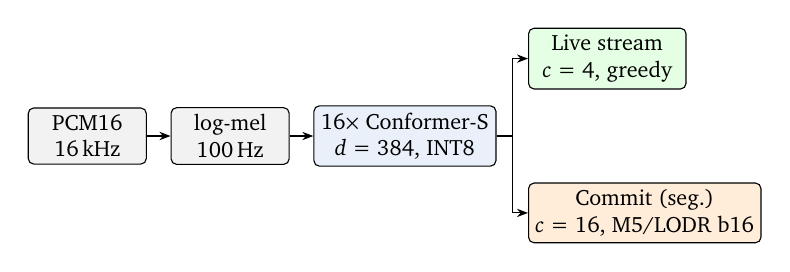
\begin{tikzpicture}[
  font=\footnotesize, >={Stealth[length=4pt]},
  blk/.style={draw, rounded corners=2pt, minimum height=6.5mm, inner sep=2.5pt, align=center},
  enc/.style={blk, fill=blue!10, minimum width=22mm},
  live/.style={blk, fill=green!10, minimum width=20mm},
  fin/.style={blk, fill=orange!15, minimum width=24mm},
  io/.style={blk, fill=gray!10, minimum width=15mm}]
\node[io] (pcm) {PCM16\\16\,kHz};
\node[io, right=3mm of pcm] (mel) {log-mel\\100\,Hz};
\node[enc, right=3mm of mel] (enc) {16$\times$ Conformer-S\\$d=384$, INT8};
\node[live, above right=2mm and 4mm of enc] (lout) {Live stream\\$c=4$, greedy};
\node[fin, below right=2mm and 4mm of enc] (fout) {Commit (seg.)\\$c=16$, M5/LODR b16};
\draw[->] (pcm) -- (mel);
\draw[->] (mel) -- (enc);
\draw[->] (enc.east) -- ++(2mm,0) |- (lout.west);
\draw[->] (enc.east) -- ++(2mm,0) |- (fout.west);
\end{tikzpicture}}
\caption{Dual operating points of \ultra{} \ReleaseVer{} on one prepared INT8 artifact: a
continuous 160\,ms live stream ($c=4$, greedy or with a compact LM) and an utterance-segmented 640\,ms commit pass
($c=16$) with 5-gram LM and LODR beam search.}
\label{fig:arch}
\end{figure}

\section{An Integer-Exact CPU Engine}\label{sec:engine}

The inference engine and commit-pass decoder are implemented in pure Rust with no ONNX Runtime,
BLAS, or external ML framework, providing scalar reference, AVX2/FMA, and ARM NEON kernels. Every
optimisation is gated on bit-identical outputs against hashed encoder projections and token
sequences.

\para{Per-row centred INT8.} Weights are quantised offline per output channel,
$w_q = \mathrm{round}(w/s_w)$ with $s_w = \max|w|/127$. Activations are quantised dynamically per
frame row, centred on that row's range:
\begin{equation}
\begin{gathered}
c = \tfrac{1}{2}(x_{\max}+x_{\min}),\qquad s_a = \tfrac{1}{254}(x_{\max}-x_{\min}),\\
x_q = \mathrm{rne}\bigl((x-c)/s_a\bigr),
\end{gathered}
\end{equation}
with $|x_q|\le 127$ and round-half-even. The linear output is recovered exactly as
\begin{equation}
y_{rn} = s_a^{(r)} s_w^{(n)} \textstyle\sum_k x_q w_q \;+\; c^{(r)} \bar w_n + b_n,
\end{equation}
where $\bar w_n = s_w^{(n)}\sum_k w_{q,nk}$ is precomputed offline, so centring adds one fused
multiply-add per output and prevents one-sided post-SiLU activations from wasting half of the INT8
dynamic range. Because each row's scale and centre depend only on that row, a stream's tokens never
depend on batch size or batch partners (verified bit-identical across batch sizes 1 to 32).

\para{Exact integer kernels and portable log-mel.} On x86 AVX2, the $4\times 16$ GEMM tile uses
\texttt{vpmaddubsw} on $(|x_q|, \mathrm{sign}(w_q, x_q))$. With $|x_q|,|w_q|\le 127$, pairwise
products sum to at most $2\cdot 127^2 = 32{,}258 < 2^{15}$, so the 16-bit step never saturates and
int32 accumulation matches the scalar reference bit for bit; ARM NEON computes the same exact sums
with \texttt{sdot}/\texttt{smmla}. To prevent 1-ULP platform \texttt{libm} differences from
flipping quantisation ties across architectures, the log-mel front end replaces platform
transcendentals with portable unfused IEEE double arithmetic (Cody--Waite range reduction,
polynomial $\sin$/$\cos$/$\log$, precomputed FFT twiddles, and sparse triangular filterbank).

\para{Native commit-pass LM/LODR decoder and parity.} The commit binary
(\texttt{ultra-engine-commit}) shares the exact same INT8 encoder and joiner, runs the live
160\,ms stream to emit provisional text, and at each utterance endpoint executes the 640\,ms
commit pass with a packed 5-gram LM (\texttt{M5.ulm}) and LODR beam-16 search.
Prepared INT8 weights are verified by SHA-256 at load time. On the prior release artifact of identical
architecture and full LibriSpeech DEV (\RelFullUtts{} utterances), prepared INT8 matched FP32 PyTorch within \RelIntEightDelta\pp pooled
WER (one-sided 95\% bootstrap bounds \RelIntEightLo{} to \RelIntEightHi\pp), well inside the
pre-registered \PreregDeltaPP\pp / \PreregUpperPP\pp gate, and produces bit-identical transcripts
across all three cold repetitions on the evaluated Zen~2 AVX2 host (\cref{tab:repro}).

\begin{table}[t]
\centering
\caption{\textbf{Verified reproducibility evidence for \ultra{} \PriorVer{}} (scoped strictly to
receipts verified on that release INT8 artifact; the \ReleaseVer{} witness decodes are in \cref{sec:candidate}).}
\label{tab:repro}
\footnotesize
\setlength{\tabcolsep}{3.5pt}
\begin{tabular}{@{}p{2.3cm}p{2.7cm}p{2.87cm}@{}}
\toprule
Property & Verified scope & Outcome \\
\midrule
INT8 vs.\ FP32 parity & Full DEV (\RelFullUtts{} utt) & \RelIntEightDelta\pp (\RelIntEightLo{} to \RelIntEightHi\pp) \\
Repeated cold runs & 730-utt DEV panel, 3 reps & 730/730 identical (live \& final) \\
Batch invariance & Batch sizes 1 to 32 & Bit-identical per-row tokens \\
Weight integrity & Prepared INT8 bundle & Verified SHA-256 at load \\
\bottomrule
\end{tabular}
\end{table}

\section{Training}\label{sec:training}

\para{Data and pseudo-labelling.} \ultra{} \PriorVer{} is trained on
LibriSpeech~\cite{panayotov2015librispeech} 960\,h combined with Libri-Light~\cite{kahn2020librilight}
(\texttt{small} and \texttt{medium} splits) pseudo-labelled by the pretrained streaming Zipformer
INT8 model (R0, which is also the Zipformer comparator in \cref{fig:money,tab:measured}). We state
this explicitly because \ultra{} \PriorVer{} is not trained on LibriSpeech 960\,h alone, and its
pseudo-labels inherit the Zipformer teacher's domain and text style. \ultra{} \ReleaseVer{} continues the same
recipe over \CandTrainKh\,h of logged audio, adding Libri-Light large; the curves below are those of \PriorVer{}.

\para{Recipe.} We optimise the joint RNN-T and auxiliary CTC loss (CTC weight \CtcWeight) with
AdamW, cosine learning-rate decay, SpecAugment~\cite{park2019specaugment}, speed perturbation, and
a small emission delay penalty (\DelayPenalty) to keep live-stream word latency low. The RNN-T loss
evaluates the joiner in time chunks without materialising the full $(B,T,U{+}1,V{+}1)$ lattice.
Training finishes with an exponential moving average (EMA)~\cite{polyak1992ema} cooldown phase,
yielding a single checkpoint whose weights are exported to prepared per-channel INT8 with zero
quantisation-aware retraining. The 5-gram language model (\texttt{M5.ulm}) used in the
utterance-segmented commit pass is trained on the standard LibriSpeech OpenSLR-11 text corpus.

% Shared pgfplots style for the Isosyll paper figures (paper-data). Okabe--Ito colour-blind-safe palette;
% every series also differs by marker shape so the figures survive greyscale printing.
% Inputs CSVs from \paperdatadir (default data/, relative to docs/paper/paper.tex).
\providecommand{\paperdatadir}{data/}%
\definecolor{okVermillion}{RGB}{213,94,0}%
\definecolor{okBlue}{HTML}{D9480F}% house accent: Isosyll is orange, never the secondary blue%
\definecolor{okGreen}{RGB}{0,158,115}%
\definecolor{okOrange}{RGB}{230,159,0}%
\definecolor{okSky}{RGB}{86,180,233}%
\definecolor{okPurple}{RGB}{204,121,167}%
\definecolor{okGrey}{RGB}{110,110,110}%
\definecolor{okInk}{RGB}{64,64,64}% neutral marks beside the accent okBlue (darker, so they differ in greyscale too)
\pgfplotsset{%
  ultra/base/.style={%
    font=\footnotesize, tick label style={font=\scriptsize}, label style={font=\footnotesize},%
    legend style={font=\scriptsize, draw=none, fill=none}, axis line style={okGrey},%
    tick style={okGrey}, major grid style={gray!25}, grid=major, clip=false,%
  },%
  ultra/rzero/.style={color=okVermillion, mark=square*, mark size=1.6pt, thick},%
  ultra/dense/.style={color=okBlue, mark=*, mark size=1.7pt, thick},%
  ultra/mr/.style={color=okGreen, mark=triangle*, mark size=2.1pt, thick},%
  ultra/failed/.style={mark options={fill=white}},%
  % keep only rows whose column #1 equals #2
  ultra/keep if/.style 2 args={x filter/.append code={%
    \edef\ultratempa{\thisrow{#1}}\edef\ultratempb{#2}%
    \ifx\ultratempa\ultratempb\else\def\pgfmathresult{inf}\fi}},%
}%
%
\begin{figure}[t]
\centering
\begin{tikzpicture}
\begin{axis}[ultra/base, width=0.97\columnwidth, height=4.6cm, xmin=0, xmax=140, ymin=5, ymax=9,
  xlabel={Cumulative training audio (thousand hours)}, ylabel={Full-DEV pooled WER (\%)},
  legend cell align=left, legend columns=2, legend style={at={(.5,-.3)}, anchor=north, column sep=4pt}]
\fill[gray!10] (axis cs:\TrainStageOneEndKhRaw,5) rectangle (axis cs:140,9);
\addplot[ultra/dense, mark options={fill=white}, ultra/keep if={series}{s1c4}]
  table[col sep=comma, x=audio_kh, y=wer] {\paperdatadir training_curve.csv};
\addlegendentry{Stage 1 live $c{=}4$}
\addplot[ultra/dense, dashed, mark=o, ultra/keep if={series}{s1c16}]
  table[col sep=comma, x=audio_kh, y=wer] {\paperdatadir training_curve.csv};
\addlegendentry{Stage 1 $c{=}16$}
\addplot[ultra/rzero, ultra/keep if={series}{s2live}]
  table[col sep=comma, x=audio_kh, y=wer] {\paperdatadir training_curve.csv};
\addlegendentry{Stage 2 live $c{=}4$ (INT8)}
\addplot[ultra/mr, ultra/keep if={series}{s2final}]
  table[col sep=comma, x=audio_kh, y=wer] {\paperdatadir training_curve.csv};
\addlegendentry{Stage 2 final (INT8)}
\node[font=\scriptsize, anchor=north west, okGrey] at (axis cs:\TrainStageOneEndKhRaw,9) {+ Libri-Light};
\end{axis}
\end{tikzpicture}
\caption{\textbf{Training dynamics of the release lineage} on full LibriSpeech DEV (\ultra{} \PriorVer{}).
Stage~1 trains on LibriSpeech 960\,h alone: live WER stops improving after about \TrainPlateauMidKh\,h
(\TrainPlateauMid\% there, \TrainPlateauEnd\% after \TrainStageOneEpochs{} epochs). Stage~2 (shaded) adds
R0-pseudo-labelled Libri-Light and an EMA cooldown, lowering live WER by \TrainLiveGain\pp and final WER by
\TrainFinalGain\pp; the gain arrives with the Libri-Light \texttt{medium} split. Stage-1 points use the PyTorch
streaming decoder, stage-2 points the INT8 engine, which matches it at the stage boundary
(\TrainEngineEnd\% vs.\ \TrainPlateauEnd\%).}
\label{fig:training}
\end{figure}
%
\para{Long-run dynamics.} The release saw \TrainTotalKh\,h of logged training audio in three stages
(\cref{fig:training}): \TrainStageOneKh\,h of LibriSpeech 960\,h (\TrainStageOneEpochs{} epochs),
\TrainStageTwoKh\,h with Libri-Light, and a \TrainCoolKh\,h EMA cooldown. On LibriSpeech alone the
model saturates: live WER is \TrainPlateauMid\% after \TrainPlateauMidKh\,h and \TrainPlateauEnd\% at
the end of stage~1, so longer training on the same 960\,h buys nothing. New audio does: Libri-Light
\texttt{small} (378\,h) moves live WER only to \TrainSmallLive\%, while adding \texttt{medium}
(3{,}396\,h) reaches \TrainMediumLive\% within ten thousand hours, and the cooldown ends at the release
point. For a model this small, the lever is data diversity, not epochs.

\section{Evaluation Protocol}\label{sec:protocol}

\para{Workload and unified scoring.} Every system in \cref{fig:money,tab:measured} decodes the
exact same staged audio: a 730-utterance LibriSpeech DEV panel (\ColdAudioMinutes\,min; 400
dev-clean utterances from 40 speakers and 330 dev-other utterances from 33 speakers, covering every
DEV speaker). Every hypothesis is scored by a single Rust scorer (\texttt{ultra-score}) and a
single text normaliser. WER pools edits and reference words over the utterance population $U$:
\begin{equation}
\mathrm{WER}(U)=100\,\frac{\sum_{i\in U}(S_i+D_i+I_i)}{\sum_{i\in U}N_i}.
\end{equation}
We report dev-clean, dev-other, and pooled panel WER for every system, plus full LibriSpeech DEV
(\RelFullUtts{} utterances) accuracy for \ultra{} \ReleaseVer{} and \PriorVer{}.

\para{Single-core timing and quiet-host guard.} For primary quiet-host comparisons, each run uses one process with one inference thread pinned to
one physical Zen~2 core, alone on its 4-core L3 complex. Across three runs, we report the median
CPU-seconds per audio-second (\cpus) and its
reciprocal, throughput in $\times$ real time, alongside peak resident memory (RSS) and artifact
size. Every primary row is measured on an otherwise idle host (H1, at most two other busy cores
during any repetition, host timers and CI paused; \cref{tab:hardware}). Comparator rows measured on
the shared host (H0) before their quiet-host H1 holds are marked interim and drawn lighter.

\begin{table}[t]
\centering
\caption{Zen~2 hosts used in the measured comparison (both AMD Threadripper PRO 3995WX).}
\label{tab:hardware}
\footnotesize
\setlength{\tabcolsep}{3pt}
\begin{tabular}{@{}lp{0.34\columnwidth}p{0.32\columnwidth}r@{}}
\toprule
Host & CPU & Memory & Rows \\
\midrule
\rawinput{data/table_hardware.tex}
\bottomrule
\end{tabular}
\end{table}

\para{Operating classes.} We separate systems by what they require to emit text: (i) \emph{live
streaming} systems emit words continuously while audio arrives without needing an endpoint;
(ii) \emph{streaming + utterance-segmented commit} (\ultra{} \ReleaseVer{} final) emits live words
and runs a second-pass commit decoder once an utterance endpoint is declared; and (iii)
\emph{offline whole-utterance} systems (Parakeet TDT v3) see the full clip before emitting a word
and are drawn hollow in \cref{fig:money}.

\para{Energy.} On the quiet host H1, CPU energy is read from the service core's RAPL energy
register during the timing run and divided by decoded audio seconds (CPU core domain only, not
wall power). The interleaved R6 rows (\ultra{} and Zipformer INT8) subtract the core idle floor
(\texttt{jsr.energy-bench/v1}, exact phase boundaries). Separately timed Moonshine, Parakeet, and
Nemotron joins use \texttt{core\_msr\_active} and include that floor, so their joules are not a
paired ratio against the R6 rows. For the \ultra{} \PriorVer{} commit pass we also record
package-domain J/audio-s.

\para{Test-set disclosure and INT8 gate.} All accuracy numbers in this paper are LibriSpeech DEV
only; no test-set numbers appear. In accordance with our benchmark freeze protocol, LibriSpeech
test-clean and test-other were read several times before the freeze, and no checkpoint selection
used test data. Prepared INT8 artifacts must pass a paired speaker-cluster
bootstrap~\cite{bisani2004bootstrap} gate against FP32 within \PreregDeltaPP\pp point delta and
\PreregUpperPP\pp one-sided 95\% upper bound. \Cref{tab:metrics} summarises all reported quantities.

\begin{table}[t]
\centering
\caption{\textbf{Measurement definitions} used consistently across figures and tables.}
\label{tab:metrics}
\footnotesize
\setlength{\tabcolsep}{3.5pt}
\begin{tabular}{@{}p{2.35cm}p{5.75cm}@{}}
\toprule
Quantity & Definition and boundary \\
\midrule
Cold throughput & Median audio-s / CPU-s across 3 cold runs on 1 pinned Zen~2 core (process tree, model load included). \\
Paced utilisation & Fraction of one core busy while serving $N$ real-time paced (20\,ms packet) live streams. \\
Active core J/audio-s & R6 rows (\ultra{}, Zipformer): service-core RAPL per audio-s with the idle floor subtracted. Moonshine, Parakeet, and Nemotron include the floor. CPU domain only, not wall power. \\
Net / gross W & Paced core power per stream with (net) or without (gross) subtracting the idle core floor. \\
Peak RSS & Peak resident memory of the full recogniser process tree (MB, $10^6$ bytes), distinct from on-disk artifact size. \\
Lag vs.\ delay & Live stable-word lag vs.\ forced-aligned word ends (128\,s continuous stream); final commit delay after utterance endpoint. \\
\bottomrule
\end{tabular}
\end{table}

\section{Results}\label{sec:results}

\subsection{All Public CPU Comparators vs.\ \ultra{}}\label{sec:compare}

\Cref{fig:money} draws live +LM at 160\,ms and the utterance-end commit pass against every timed
public comparator. \Cref{tab:measured} keeps those two rows plus the 320\,ms and greedy modes of the
same 60\,MB INT8 artifact, beside all \ColdCompleteCompCount{} public open-weights CPU comparators
with complete 730-utterance LibriSpeech DEV panel WER. \ColdHostSentence{} \ColdSubsetSentence{} \ColdOrderSentence{}

\para{Speed and lowest-power operating points.} \ColdHeadSentence{} On the exact same weights, matching
Zipformer INT8's 320\,ms chunk length (\ultra{} live +LM, 320\,ms) yields our lowest active-core energy
and best live WER at \VsWideSpeed$\times$ real time, \VsWideWatts\,J per audio-second, and \VsWideWer\%
panel WER (\CandLiveLmEightFullWer\% full DEV)---\VsWideSpeedX$\times$ Zipformer's paired throughput at
\VsWideEnergyPct\% of its active core energy. Greedy 160\,ms live decoding reaches \VsGreedySpeed$\times$
real time in \ColdRcTwoLiveGreedyRss\,MB RAM at \VsGreedyWatts\,J per audio-second (\VsGreedyWer\% panel
WER). At utterance endpoints, the commit pass runs at \ColdFinalCorePct\% of one quiet Zen~2 core
(\ColdFinalVsZipSpeed{}).

\para{Accuracy.} \ColdAccuracySentence{} Notably, while \ultra{} uses Libri-Light pseudo-labels
generated by the Zipformer comparator (R0), its utterance-segmented commit pass matches streaming
Zipformer INT8's pooled panel WER (\ColdHeadWer\% vs.\ \ColdZipWer\%, \VsVerdictTwo{} it under the
paired test of \cref{sec:versus}), with lower dev-other WER (\ColdHeadWerOther\% vs.\ \ColdZipWerOther\%)
and equal dev-clean WER (\ColdHeadWerClean\% vs.\ \ColdZipWerClean\%). Larger 600M-parameter models
achieve lower WER at much higher CPU and energy cost (offline Parakeet TDT v3 on quiet H1; Nemotron
560\,ms on the quiet 73-clip timing subset; Parakeet unified stream 160\,ms on Xeon~8358).
\RelSubsetNote{}

\para{Memory and active-core energy.} \ColdMemorySentence{} \ColdWattsSentence{} The bottom panel of
\cref{fig:money} draws only the matched R6 rows: live +LM is \ColdLiveWatts\,J per audio-second,
\VsEnergyPctOne\% of Zipformer INT8 (\ColdZipRsixWatts\,J) on the same blocks, with the idle floor
subtracted. The commit pass is \ColdHeadWatts\,J per audio-second. Moonshine, Parakeet, and Nemotron
joules in \cref{tab:measured} include the core idle floor and are not a paired ratio. The 320\,ms and
greedy rows in \cref{tab:measured} are \VsWideWatts\,J and \VsGreedyWatts\,J.

\subsection{Head-to-Head with Zipformer INT8}\label{sec:versus}

Zipformer INT8 is the strongest public streaming comparator near our cost point and the teacher of our
pseudo-labels, so we compare against it directly on the same utterances and the same core
(\cref{tab:versus}), timed in the same three interleaved blocks on quiet H1; speed, energy and memory
ratios are medians of the within-block ratios. WER differences are paired with speaker-cluster
bootstrap. Because the 730-utterance panel overlaps the selection half of DEV, we always report the
unselected confirmation half (C, \CandCUtts{} utterances; \cref{sec:candidate}) beside it: on C, live
+LM trails Zipformer by \CandLiveLmEightCDelta\pp (320\,ms, bounds \CandLiveLmEightCLo{} to
\CandLiveLmEightCHi) and \CandLiveLmCDelta\pp (160\,ms, bounds \CandLiveLmCLo{} to \CandLiveLmCHi).
The 160\,ms live stream uses \VsCpuPctOne\% of Zipformer's CPU time (\VsSpeedXOne$\times$ throughput),
\VsEnergyPctOne\% of its active core energy, and \VsRssPctOne\% of its memory with half the chunk
(\VsChunkOne\,ms vs.\ \VsZipChunk\,ms); its panel WER is \VsVerdictOne{} Zipformer's (\VsDeltaOne\pp,
bounds \VsLoOne{} to \VsHiOne\pp). The final commit pass on the same weights is \VsVerdictTwo{}
Zipformer's (\VsDeltaTwo\pp, bounds \VsLoTwo{} to \VsHiTwo\pp; \CandFinalCDelta\pp on C) at
\VsSpeedXTwo$\times$ its single-core speed and \VsEnergyPctTwo\% of its active core energy.

\begin{table}[t]
\centering
\caption{\textbf{Head-to-head with Zipformer INT8}: same 730 DEV utterances (the selection panel; the unselected-half gaps are in \cref{sec:candidate}), same quiet Zen~2 core, same interleaved blocks, median of three. Ratios are medians of within-block ratios. $\Delta$ is paired (speaker-cluster bootstrap); negative means fewer errors. \textsuperscript{a}Live stream plus a commit pass at reference utterance boundaries.}
\label{tab:versus}
\footnotesize
\setlength{\tabcolsep}{1.5pt}
\begin{tabular}{@{}lrrr@{}}
\toprule
Metric & Zipformer & \ultra{} live & \ultra{} final \\
\midrule
Live chunk (ms) & 320 & 160 & 160\textsuperscript{a} \\
Pooled WER (\%) & 5.25 & 5.54 & 5.00 \\
$\Delta$ WER vs.\ Zip.\ (pp) & --- & +0.28 & $-$0.26 \\
\quad one-sided 95\% bounds & --- & [$-$0.02, +0.58] & [$-$0.57, +0.05] \\
1-core speed ($\times$ RT) & 14.0 & 32.7 & 16.8 \\
J per audio-s (core) & 0.573 & 0.328 & 0.661 \\
Peak RSS (MB) & 152 & 109 & 387 \\
\bottomrule
\end{tabular}
\end{table}


\subsection{Registered Look and Cross-ISA Reproducibility}\label{sec:candidate}

The \ReleaseVer{} acoustic model (RC2, identical weights in v3.2.0) was trained on \CandTrainKh\,h of
logged audio (adding Libri-Light large to the lineage) and frozen before one registered look on the
panel and the unselected C half (\CandCUtts{} utterances; \cref{tab:candidate}). On the panel, the
160\,ms live +LM stream trails Zipformer by \CandLiveLmPanelDelta\pp (upper \CandLiveLmPanelHi\pp), so
non-inferiority at the registered \CandNiMargin\pp margin is not shown (Holm-adjusted
$p=\CandHolmNi$); on C the gap is \CandLiveLmCDelta\pp (320\,ms: \CandLiveLmEightCDelta\pp). The final
pass reaches \CandFinalWer\% on the panel (\CandFinalCDelta\pp vs.\ Zipformer on C; Holm-adjusted
$p=\CandHolmFinal$). RC2 made \CandFinalFullEdits{} full-DEV final edits against a registered adoption
gate of \CandGateFinalFull{} and missed both panel edit targets (\CandGateLivePanel{} live,
\CandGateFinalPanel{} final). \ultra{} \ReleaseVer{}/v3.2.0 is released by owner decision with these
misses stated explicitly.

\ultra{} preserves exact cross-architecture reproducibility: \CandIsaRuns{} witness decodes on Intel
Xeon (AVX2 and AVX-512 VNNI) and Apple M3 (NEON) across live greedy, both live LM policies, and the
final pass reproduce the Zen~2 transcripts on all \ScalarUtts{} panel utterances. On main from
\ScalarMainCommit{} (including v3.2.0), a forced scalar reference backend also gives
\ScalarDiffs/\ScalarUtts{} differing utterances across AVX2, AVX-512 VNNI, NEON, and scalar.

\begin{table*}[t]
\centering
\caption{\textbf{RC2 (released as v3.1.0), single registered look.} It missed its registered gates and is released by owner decision, not as a gate pass. $\Delta$ is RC2 minus Zipformer INT8 (or minus shipped v3.0.0) on the same utterances, with one-sided 95\% bounds from the pinned scorer; negative means fewer errors. The 730-utterance panel overlaps the half of DEV used for selection; the C half (2,785 utterances) was never used for selection. Full-DEV WER is descriptive. Live rows compare with shipped v3.0.0 live greedy (160\,ms); the final rows with its final pass. Final rows run the 160\,ms live stream and commit with a 640\,ms chunk at reference utterance boundaries.}
\label{tab:candidate}
\footnotesize
\setlength{\tabcolsep}{4pt}
\begin{tabular}{@{}lrrrlll@{}}
\toprule
Mode & Chunk (ms) & Panel WER & Full-DEV WER & $\Delta$ vs.\ Zip.\ (panel) & $\Delta$ vs.\ Zip.\ (C half) & $\Delta$ vs.\ v3.0.0 (panel) \\
\midrule
Live, greedy & 160 & 6.23 & 6.83 & +0.98 [+0.66, +1.29] & +1.59 [+1.31, +1.90] & $-$0.62 [$-$0.86, $-$0.38] \\
Live + 34.5\,MiB LM & 160 & 5.54 & 6.10 & +0.28 [$-$0.02, +0.58] & +0.81 [+0.62, +1.02] & $-$1.31 [$-$1.63, $-$1.00] \\
Live + 34.5\,MiB LM & 320 & 5.50 & 5.87 & +0.24 [$-$0.04, +0.52] & +0.65 [+0.47, +0.84] & $-$1.35 [$-$1.68, $-$1.03] \\
Final, M5 LM & 640 & 5.00 & 5.22 & $-$0.26 [$-$0.57, +0.05] & $-$0.11 [$-$0.35, +0.11] & $-$0.06 [$-$0.28, +0.17] \\
Final, 146.8\,MiB LM & 640 & 5.09 & 5.24 & $-$0.17 [$-$0.49, +0.15] & $-$0.10 [$-$0.35, +0.12] & --- \\
\midrule
Zipformer INT8 & 320 & 5.25 & 5.37 & --- & WER 5.13 & --- \\
\bottomrule
\end{tabular}
\end{table*}


\subsection{Quiet-Speech Level Normalisation (v3.2.0 \texttt{-{}-rms-norm})}\label{sec:level}

The runtime-only v3.2.0 release (build commit \VThreeTwoBuildCommit{}, signed tag \VThreeTwoTagObject{},
keeping identical \ReleaseVer{} RC2 weights) adds an opt-in final-pass RMS level normaliser
(\texttt{-{}-rms-norm}, off by default). On the unselected DEV confirmation half (C) with the frozen M5
commit pass, \texttt{-{}-rms-norm} left native 0\,dB accuracy unchanged within noise
(\AudioZOneCleanDelta\pp, one-sided 95\% upper \AudioZOneCleanUpper\pp) while improving synthetic
$-$20\,dB and $-$30\,dB attenuated speech by \AudioZOneTwentyDelta\pp (upper \AudioZOneTwentyUpper\pp)
and \AudioZOneThirtyDelta\pp (upper \AudioZOneThirtyUpper\pp). On automatic-endpoint chapter streams
(DEV selection half S, 90 chapters, verifying hangover, EOF, deadline, and PCM-cap triggers), it changed
pooled WER by \AudioZOneAutoCleanDelta\pp at 0\,dB, \AudioZOneAutoTwentyDelta\pp at $-$20\,dB, and
\AudioZOneAutoThirtyDelta\pp at $-$30\,dB (uppers \AudioZOneAutoCleanUpper{},
\AudioZOneAutoTwentyUpper{}, and \AudioZOneAutoThirtyUpper\pp). Paired pinned-core H0 relative CPU
overhead stayed within \AudioZOneCpuEngineUpper\% for the commit binary and \AudioZOneCpuStreamUpper\%
for stream commit mode, with \AudioZOneCrossIsaDiffs/\AudioZOneCrossIsaClips{} committed-text
differences across AVX2, scalar, and NEON on the \AudioZOneCrossIsaCommit{} cross-ISA witness builds
(\AudioZOneOracleTupleDiffs/\AudioZOneCrossIsaClips{} full-tuple differences vs.\ the independent
oracle with flag on, \AudioZOneCrossIsaDiffs{} committed-text differences).

\subsection{Full-DEV Accuracy and INT8 Parity}\label{sec:fulldev}

\Cref{tab:fulldev} reports full LibriSpeech DEV (\RelFullUtts{} utterances: \CandFullCleanUtts{}
dev-clean and \CandFullOtherUtts{} dev-other) accuracy for all four modes of our single 60\,MB INT8
artifact under the same unified scorer. Full DEV contains the selection half, so these numbers are
descriptive. On the prior release artifact of identical architecture, prepared INT8 matched FP32 PyTorch
across all \RelFullUtts{} utterances within \RelIntEightDelta\pp pooled WER (one-sided 95\%
speaker-cluster bootstrap bounds \RelIntEightLo{} to \RelIntEightHi\pp), well inside the pre-registered
parity gate.

\begin{table}[t]
\centering
\caption{\textbf{Full LibriSpeech DEV (\RelFullUtts{} utterances)} WER (\%) across all four operating
points of our single 60\,MB INT8 artifact (unified \texttt{ultra-score}).}
\label{tab:fulldev}
\footnotesize
\setlength{\tabcolsep}{3pt}
\begin{tabular}{@{}lrrr@{}}
\toprule
Mode (same INT8 weights) & dev-clean & dev-other & Pooled \\
\midrule
Live greedy (160\,ms, $c=4$) & \CandLiveGreedyFullClean & \CandLiveGreedyFullOther & \CandLiveGreedyFullWer \\
Live +LM (160\,ms, $c=4$) & \CandLiveLmFullClean & \CandLiveLmFullOther & \CandLiveLmFullWer \\
Live +LM (320\,ms, $c=8$) & \CandLiveLmEightFullClean & \CandLiveLmEightFullOther & \CandLiveLmEightFullWer \\
\textbf{Final commit (640\,ms, M5)} & \textbf{\CandFinalFullClean} & \textbf{\CandFinalFullOther} & \textbf{\CandFinalFullWer} \\
\bottomrule
\end{tabular}
\end{table}

\subsection{Paced Always-On Live Capacity on One Quiet Zen~2 Core}\label{sec:capacity}

To measure real-time always-on capacity and stable-word lag under live packet pacing, we run
$N\in\{1,4,8,16\}$ concurrent live streams (\texttt{ultra stream}, real-time pacing, 20\,ms packets,
per-packet wakes) pinned to a single quiet Zen~2 core on the prior release artifact of identical
compute cost (\cref{tab:capacity}). Sixteen simultaneous live streams occupy \RelCapSixteenBusy\% of one
core at \RelCapSixteenNetW\,W net (\RelCapSixteenGrossW\,W gross) core power per stream and stable-word
lag \RelCapSixteenLagPfifty/\RelCapSixteenLagPninetyFive\,ms (p50/p95). A lone paced stream costs more
per stream (\RelCapOneNetW\,W net, \RelCapOneBusy\% busy) because it wakes an otherwise idle core at the
packet rate and amortises model load over a single 128\,s stream.

\begin{table}[t]
\centering
\caption{\textbf{Always-on live capacity on one quiet Zen~2 core}
(real-time pacing, 20\,ms packets, continuous 128\,s stream of 22 DEV clips; prior release artifact of
identical per-frame cost). Net W subtracts the idle core floor; gross W is total core power divided by $N$.}
\label{tab:capacity}
\footnotesize
\setlength{\tabcolsep}{3.5pt}
\begin{tabular}{@{}rrrr@{}}
\toprule
Streams ($N$) & Core busy (\%) & Net / gross W & Lag p50 / p95 (ms) \\
\midrule
1 & \RelCapOneBusy & \RelCapOneNetW{} / \RelCapOneGrossW & \RelCapOneLagPfifty{} / \RelCapOneLagPninetyFive \\
4 & \RelCapFourBusy & \RelCapFourNetW{} / \RelCapFourGrossW & \RelCapFourLagPfifty{} / \RelCapFourLagPninetyFive \\
8 & \RelCapEightBusy & \RelCapEightNetW{} / \RelCapEightGrossW & \RelCapEightLagPfifty{} / \RelCapEightLagPninetyFive \\
\textbf{16} & \textbf{\RelCapSixteenBusy} & \textbf{\RelCapSixteenNetW{} / \RelCapSixteenGrossW} & \textbf{\RelCapSixteenLagPfifty{} / \RelCapSixteenLagPninetyFive} \\
\bottomrule
\end{tabular}
\end{table}

\section{Limitations}\label{sec:limitations}

\para{Utterance-segmented final mode and memory.} \ColdLimitLive{} Shrinking LM memory
(\LmPackMb\,MB on disk) and commit CPU without losing accuracy remains future work.

\para{Live accuracy and next lever.} The endpoint-free live stream trades accuracy for extreme speed and
low power: its gap to Zipformer INT8 on the unselected DEV C half is \CandLiveLmCDelta\pp at 160\,ms
and \CandLiveLmEightCDelta\pp at 320\,ms (\cref{sec:candidate}). Error analysis shows that \VfDiagInteriorPct\%
of live repair positions (\VfDiagInterior{} of \VfDiagPositions{}) are common interior words on hard audio
(\texttt{dev-other}), and follow-up probes of reranking, regularisation, and relabelling existing audio
did not move clean live WER; breaking further at the same single-core compute budget will require fresh
acoustic diversity and stronger non-Zipformer supervision.

\para{Training data and LM overlap.} \ultra{} is trained on LibriSpeech 960\,h plus Libri-Light
pseudo-labelled by R0 (the Zipformer comparator). Release comparisons use read English LibriSpeech DEV
audio, which is in-domain for both \ultra{} and Zipformer; rankings on conversational, accented, or
noisy speech may differ. The OpenSLR-11 training text of \texttt{M5.ulm} contains \LmOverlapCount{} of
the \LmOverlapOf{} longer DEV transcripts verbatim; removing them leaves the relative LM WER gain
unchanged.

\para{Host coverage, energy scope, and DEV-only claims.} \ColdHostSentence{} \ColdSubsetSentence{}
Shared-host (H0) rows stay marked interim until quiet H1 holds complete. Energy measurements are
active core (CPU-domain) joules per audio-second from RAPL registers, never board or wall power.
The R6 rows subtract the core idle floor; separately timed Moonshine, Parakeet, and Nemotron joins
include it. They are measured unpaced. All accuracy numbers are LibriSpeech DEV only; as disclosed in
\cref{sec:protocol}, LibriSpeech test-clean and test-other were read several times before our
benchmark freeze, and no test-set numbers appear here.

\section{Conclusion}\label{sec:conclusion}

An always-on speech recogniser should barely register on the CPU and energy budget of its host. We
presented \ultra{}, a compact streaming Conformer transducer and pure-Rust integer-exact CPU engine
evaluated directly against all \ColdCompleteCompCount{} complete-panel public open-weights CPU
comparators on the same 730-utterance LibriSpeech DEV panel. From one \ColdHeadModel\,MB INT8 artifact on one
pinned quiet Zen~2 core, \ultra{} delivers live streaming at \ColdLiveSpeed$\times$ real time and
\ColdLiveWatts\,J/audio-s (\ColdLiveWer\% panel / \CandLiveLmFullWer\% full DEV, \ColdLiveRss\,MB RAM
at 160\,ms) and an utterance-end commit pass reaching \ColdHeadWer\% panel WER (\CandFinalFullWer\%
full DEV) at \ColdHeadSpeed$\times$ real time. The same weights also run at \VsWideSpeed$\times$ and
\VsWideWatts\,J/audio-s with a 320\,ms chunk, and greedy decoding reaches \VsGreedySpeed$\times$
(\ColdRcTwoLiveGreedyRss\,MB RAM). Transcripts reproduce bit-identically across \CandIsaRuns{} x86 and
ARM witness decodes, and sixteen paced live streams fit on one core at \RelCapSixteenBusy\% load
(\RelCapSixteenNetW\,W net per stream). \ultra{} is released by owner decision after missing its
registered full-DEV final edit gate (\CandFinalFullEdits{} vs.\ \CandGateFinalFull) and trails
Zipformer INT8 on unselected DEV live streams (\CandLiveLmCDelta\pp at 160\,ms,
\CandLiveLmEightCDelta\pp at 320\,ms). All results are exploratory and use development data only.


\bibliographystyle{plainnat}
\bibliography{refs}

\end{document}
